\chapter{Communication between Software and Arduino}
\thispagestyle{empty}
\label{sec:sw-env}

\newcommand{\LocSWfig}{\Origin/user-code/sw-env/figures}
\newcommand{\LocSWscicode}{\Origin/user-code/sw-env/scilab}
\newcommand{\LocSWscibrief}[1]{{\texttt
                  Origin/user-code/sw-env/scilab/#1}, see \fnrefp{fn:file-loc}}
\newcommand{\LocSWardcode}{\Origin/user-code/sw-env/arduino}
\newcommand{\LocSWardbrief}[1]{{\tt \seqsplit{
                        Origin/user-code/sw-env/arduino/#1}}, see \fnrefp{fn:file-loc}}

\newcommand{\LocSWchkcode}{\Origin/tools/scilab}
\newcommand{\LocSWchkbrief}[1]{{\tt \seqsplit{
                        Origin/tools/scilab/#1}}, see \fnrefp{fn:file-loc}}
\newcommand{\LocSWfirmcode}{\Origin/tools/arduino-firmware}
\newcommand{\LocSWfirmbrief}[1]{{\tt \seqsplit{
                        Origin/tools/arduino-firmware/#1}}, see \fnrefp{fn:file-loc}}

\newcommand{\LocFIMpycode}{\Origin/tools/python}  %added for python
\newcommand{\LocFIMpybrief}[1]{{\tt \seqsplit{%
                        Origin/tools/python/#1}}, see \fnrefp{fn:file-loc}} % added for python


\newcommand{\LocFIMjuliacode}{\Origin/tools/julia}  %added for julia
\newcommand{\LocFIMjuliabrief}[1]{{\tt \seqsplit{%
                        Origin/tools/julia/#1}}, see \fnrefp{fn:file-loc}} % added for julia

%%%%%%OpenModelica Starts
\newcommand{\LocFIMOpenModelicacode}{\Origin/tools/openmodelica/windows/}  %added for OpenModelica
\newcommand{\LocFIMOpenModelicabrief}[1]{{\tt \seqsplit{%
                        Origin/tools/openmodelica/windows/#1}}, see \fnrefp{fn:file-loc}} % added for OpenModelica

%%%%%OpenModelica Ends


In this chapter, we shall briefly walk through the software
environment that needs to be set up before we could start with the
\arduino\ board-based experiments. We shall start with the \arduino\
compatible Integrated Development Environment (IDE), termed as Arduino
IDE, that would be used to load the firmware on to the
microcontroller. The firmware to be loaded could be developed to serve
different purposes as per the requirement. For example, 
\begin{itemize}
      \item To run \arduino\ stand-alone, without waiting for any commands
            from other software or hardware, for the specified time or until
            power off
      \item To decode the commands sent by other software, such as Scilab, Python, 
            Julia, OpenModelica, etc., through a serial port, and 
            execute the given instructions %\item Combination of the above two
\end{itemize}
Next, we shall discuss Scilab and Xcos, which are open-source software
tools, and a related toolbox that can communicate with \arduino\ 
over a serial port using RS232 protocol. Subsequently, we shall discuss 
other open-source software tools such as Python, Julia, and OpenModelica. 

\section{Arduino IDE}\label{arduino-ide}
\label{sec:ard-start}
Arduino development environment is compatible with popular desktop
operating systems. In this section, we will learn to set up this tool
for the computers running Microsoft Windows or Linux. Later, we shall
explore the important menu options in the Arduino IDE and run a sample
program.  The following two steps have to be followed whatever operating
system is used:

\begin{enumerate}
      \item To begin, we need an \arduino\ board with a USB cable (A plug to
            B plug) as shown in \figref{arduino}.
      \item Connect it to a computer and power it up. The moment you connect \arduino\
            to the computer, an on-board power LED will turn ON.
\end{enumerate}

\subsection{Downloading and installing on Windows}
First, carry out the steps numbered 1 and 2 given above.
Starting from download, we shall go through the steps to set up
Arduino IDE on Windows OS:

\begin{enumerate}
      \setcounter{enumi}2
      \item Visit the URL, {\tt https://www.arduino.cc/en/software}. On the 
            right right side of the page, locate the link \emph{Windows ZIP file} and click on it.  
            This may redirect you to the download/donate page. Read the instructions and proceed with the
            download.
      \item Extract the downloaded ZIP file to Desktop. Do not alter any
            file or directory structure.
      \item Click on the Windows Start Menu, and open up the ``Control
            Panel''.
      \item While in the Control Panel, navigate to ``System and Security'',
            click on ``System'' and then choose the ``Device Manager''.
      \item Look for ``Other devices'' in the ``Device Manager'' list,
            expand and locate ``Unknown device''.  This may be similar to what
            is shown in \figref{win-device-manager}. In case, you don't see  
            ``Unknown device,'' look for ``Ports (COM \& LPT)'' and expand it to locate 
            ``USB Serial Device (COM2)''.
            This may be similar to what is shown in \figref{win-device-manager-com}.
      \item Right-click on the ``Unknown device'' (or ``USB Serial Device (COM2)'' as shown in 
            the previous step) and select the ``Update Driver Software'' (or ``Update driver'') option 
            as shown in \figref{win-dri-update}. 
      \item Next, choose the ``Browse my computer for Driver software''
            option.
      \item Navigate to the newly extracted Arduino folder on the Desktop and
            select ``drivers'' folder.
      \item Windows will now finish the driver installation. The Arduino IDE
            is ready for use.
\end{enumerate}
To launch Arduino IDE, browse to extracted Arduino folder on the Desktop and double click on ``arduino.exe''.
\begin{figure}
      \centering
      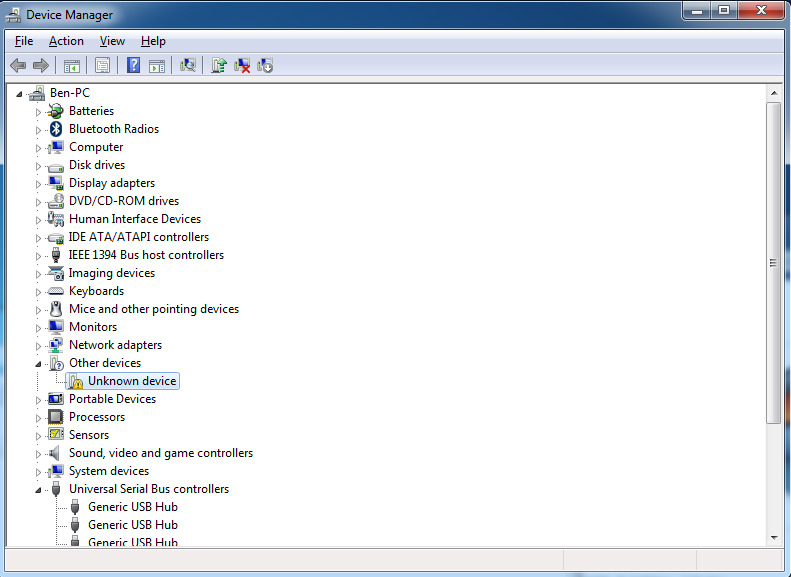
\includegraphics[width=\linewidth]{\LocHWfig/hw-device-manager.jpg}
      \caption{Windows device manager}
      \label{win-device-manager}
\end{figure}

\begin{figure}
      \centering
      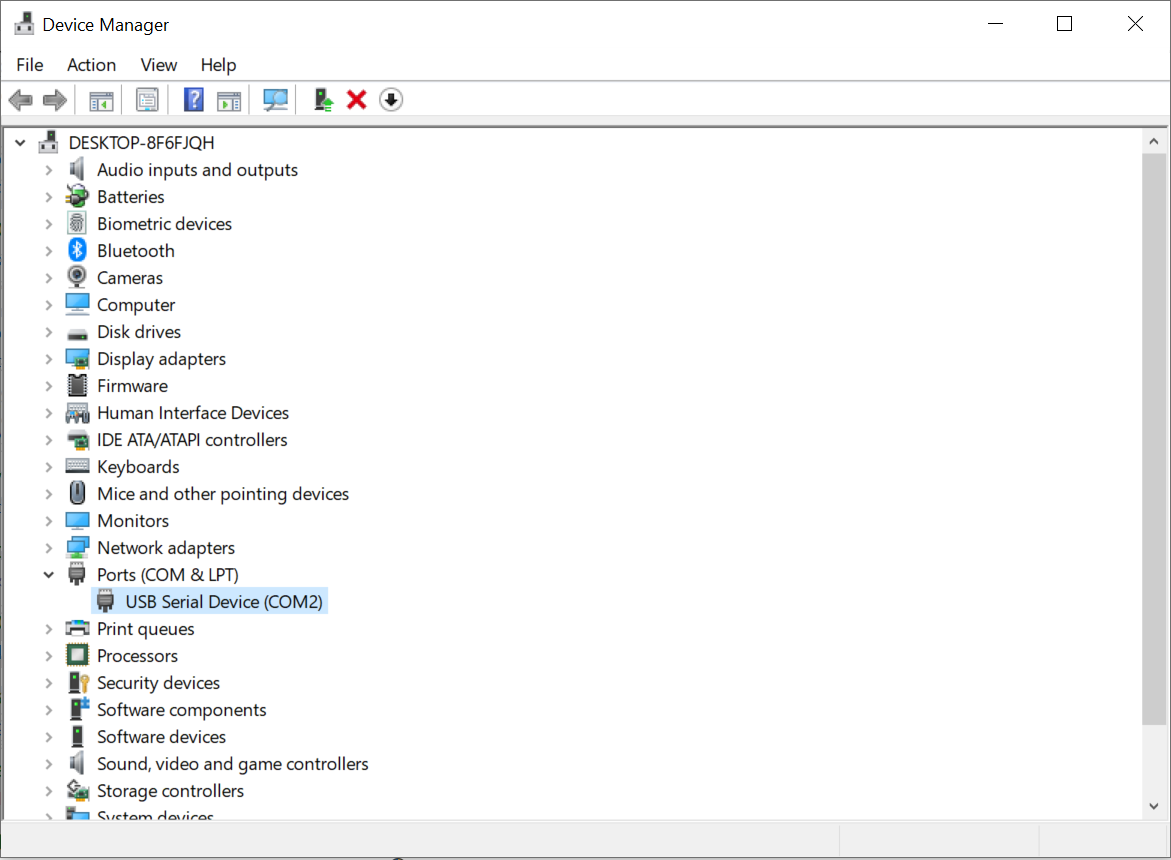
\includegraphics[width=\linewidth]{\LocSWfig/device-manager-com.png}
      \caption{Windows device manager}
      \label{win-device-manager-com}
\end{figure}

\begin{figure}
      \centering
      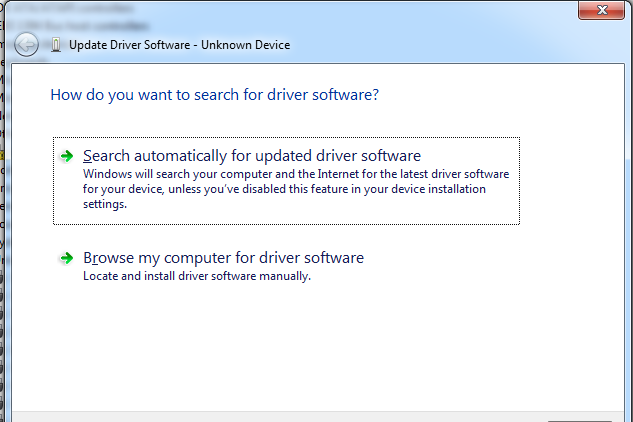
\includegraphics[width=\linewidth]{\LocHWfig/update-driver.png}
      \caption{Windows update driver option}
      \label{win-dri-update}
\end{figure}


\subsection{Downloading and installing on GNU/Linux Ubuntu}
We will now explain the installation of Arduino software on the
GNU/Linux operating system. We shall perform the installation on the 64-bit 
Ubuntu 18.04 LTS operating system.  These
instructions will work for other GNU distributions too, with little or
no modification.  First, carry out the steps numbered 1 and 2 given
above.  Then carry out the following:

\begin{enumerate}
      \setcounter{enumi}2
      \item First, update your system. Open the terminal emulator, type,
            {\tt sudo apt-get update} and press Enter. 
      \item Find out your operating system support for 64-bit
            instructions. Open the terminal emulator and type, {\tt uname -m}
      \item If it returns ``x86\_64'', then your computer has 64-bit
            operating system.   There is no visible performance difference in 32
            and 64-bit Arduino versions.
      \item Download the suitable Arduino Software version (32 or 64-bit)
            from \\ {\tt https://www.arduino.cc/en/software}.  As mentioned
            earlier, we will perform experiments with a 64-bit installation.
            
      \item At the time of writing this book, we worked with version 1.8.13.
            Assuming that you have downloaded the tar file in 
            the Downloads directory, execute the following
            commands on the terminal:
            \begin{quote}
                  {\tt cd {\large\textasciitilde}/Downloads\\
                        tar -xvf arduino-1.8.13-linux64.tar.xz\\
                        sudo mv arduino-1.8.13 /opt}
            \end{quote}
            
      \item In the same terminal session, install the required Java Runtime
            Environment with a command like,
            {\tt sudo apt-get -y install openjdk-8-jre}
            
      \item \label{itm:port-check} Execute the
            following command on the terminal to list the serial port number.\\
            {\tt ls /dev/ttyACM*}\\
            Note down the serial device filename.  Suppose that it
            is {\tt ttyACM0}.
      \item \label{itm:port-access} To make the USB port available to all users, set the read-write
            permission to the listed port:
            {\tt sudo chmod a+rw /dev/ttyACM0}. Each time you plug the \arduino\
            into the computer, you need to execute the commands given in the steps 
            numbered \ref{itm:port-check} and \ref{itm:port-access}. 
            
      \item \label{itm:create-shortcut} Create a shortcut on the desktop:\\
            {\tt cd {\large \textasciitilde}/Desktop\\
            ln -s /opt/arduino-1.8.13/arduino}
      \item \label{itm:give-permission} Give executable permission to this file through the following
            command on the terminal: {\tt chmod +x arduino}
            %   Ubuntu opens executable text files with an editor instead of
            %   executing them. To be able execute a file, open the ``Files''
            %   program from the launcher, go to menu ``Edit'', ``Preferences'', tab
            %   ``Behavior'' and set ``Executable Text Files'' to ``Ask each time'',
            %   as shown in \figref{ard-lin-executable}.
            
\end{enumerate}
% \begin{figure}
%   \centering
%   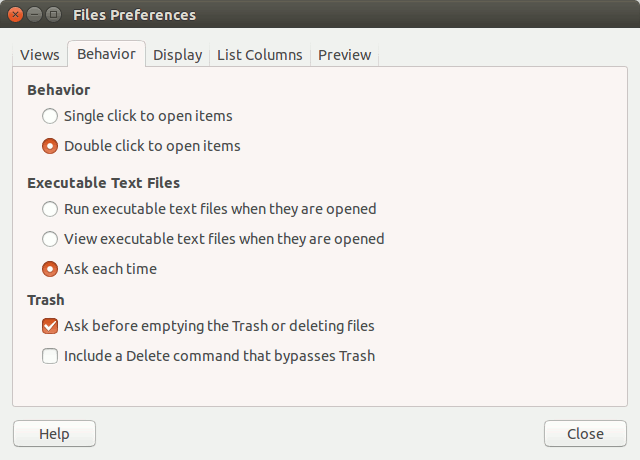
\includegraphics[scale=0.5]{\LocHWfig/executable.png}
%   \caption{Executable permission to Arduino IDE}
%   \label{ard-lin-executable}
% \end{figure}
Then double click the Arduino shortcut on the Desktop and, click ``Run''
in the dialog window to start the Arduino IDE. The dialog box is shown in \figref{ard-lin-run} for reference.
\begin{figure}
      \centering
      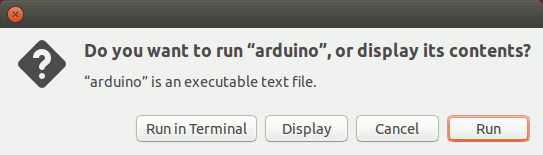
\includegraphics[scale=0.5]{\LocHWfig/run.png}
      \caption{Confirmation for executing Arduino script}
      \label{ard-lin-run}
\end{figure}
The Arduino IDE is now ready for use. There are chances that you might not 
get the Arduino shortcut on your Desktop after executing the commands given in 
steps numbered \ref{itm:create-shortcut} and \ref{itm:give-permission}. 
In that case, you can navigate into the {\tt /opt/} directory and execute the 
commands as given in \figref{arduino-opt} to start the Arduino IDE. 

\begin{figure}
      \centering
      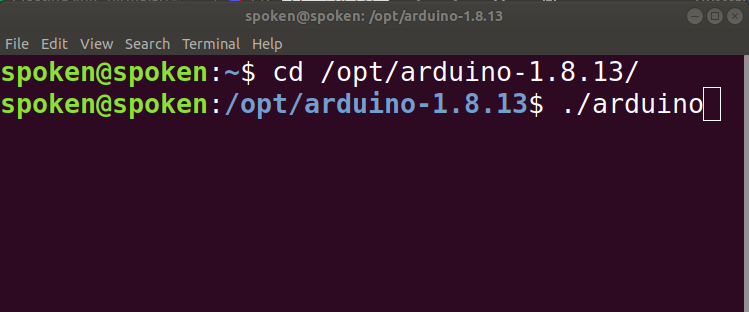
\includegraphics[width=\lgfig]{\LocSWfig/launch-arduino-opt.png}
      \caption{Linux terminal to launch Arduino IDE}
      \label{arduino-opt}
\end{figure}


\subsection{Arduino Development Environment}
\label{sec:Arduino-IDE}
The Arduino development environment, as shown in \figref{ard-ide},
consists of 
a text editor for writing code, a message area, a text console, a
toolbar with buttons for common functions, and a series of menus. It
connects to the Arduino hardware to upload programs and communicate
with them.

\begin{figure}
      \centering
      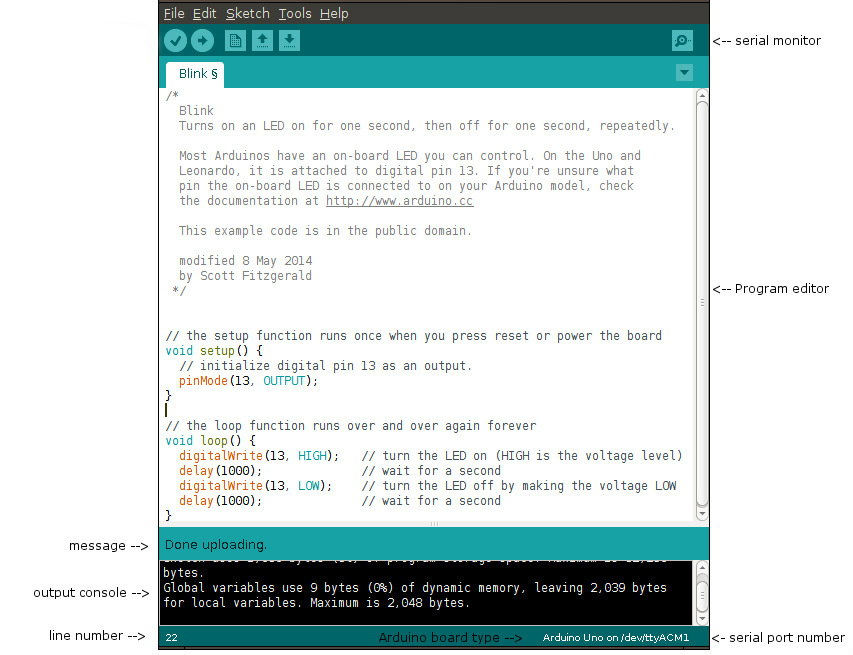
\includegraphics[width=\linewidth]{\LocHWfig/arduino-ide.jpg}
      \caption{Arduino IDE}
      \label{ard-ide}
\end{figure}
Software written using Arduino is called sketches. These sketches are
written in the text editor. Sketches are saved with the file extension
``.ino''. The frequently used icons shown in the toolbar, below the menu bar, are explained next. The names of these icons can be viewed by hovering the mouse pointer over each of them.

\begin{enumerate}
      \item Verify: Checks your code for errors
      \item Upload: Compiles your code and uploads it to the Arduino I/O
            board
      \item New: Creates a new sketch
      \item Open: Presents a menu of all the sketches in your
            sketchbook - clicking one will open it within the current window
      \item Save: Saves your sketch
      \item Serial Monitor: Opens the serial port window - the location of
            this is shown in the top right-hand corner of \figref{ard-ide}
\end{enumerate}
Note that these appear from left to right in the editor window. Next, we shall go through the additional useful options under the menu.
\begin{enumerate}
      \item File
            \begin{enumerate}
                  \item Examples: Examples that come at the time of installation
                  \item Page Setup: Configures the page parameters for the printer
                  \item Preferences: Customizes font, language, and other parameters for
                        the IDE
            \end{enumerate}
      \item Sketch
            \begin{enumerate}
                  \item Include Library: Adds a library to your sketch by inserting {\tt
                                    \#include} statements at the start of your code
            \end{enumerate}
      \item Tools
            \begin{enumerate}
                  \item Auto Format: Indents code so that opening and closing curly
                        braces line up
                  \item Archive Sketch: Archives a copy of the current sketch in .zip
                        format. The archive is placed in the same directory as the sketch.
                  \item Board: Selects the board that you're using
                  \item Port: This menu contains all the serial devices (real or
                        virtual) on your machine. It should automatically refresh every time
                        you open the top-level tools menu.
                  \item Programmer: This can be used to select a hardware programmer when programming a board or chip and not using the onboard USB-serial
                        connection. Normally you won't need this, but if you're burning a
                        bootloader to a new microcontroller, you will use this.
                  \item Burn Bootloader: The items in this menu allow you to burn a
                        bootloader onto the microcontroller on an Arduino board. This is not
                        required for normal use of an Arduino board but is useful if you
                        purchase a new ATmega microcontroller (which normally comes without a
                        bootloader). Ensure that you've selected the correct board from the
                        Boards menu before burning the bootloader.
            \end{enumerate}
\end{enumerate}

\subsection{Testing Arduino with a sample program}
\label{sec:testing-arduino}
Now, as we have a basic understanding of Arduino IDE, let us try an
example program.
\begin{enumerate}
      \item Open the Arduino IDE by clicking the shortcut ``arduino'' from
            Desktop in Ubuntu. In MS Windows browse to extracted Arduino folder
            on Desktop and double click on ``arduino.exe''.
      \item In the Arduino IDE, to know the path of your sketch files,
            navigate to File, then Preferences and then locate the ``Sketchbook
            location'' text box at the top.  You may change the path of your
            storage location. In this book, we will keep it unchanged. The path
            will be different for Windows and Ubuntu.
      \item To load a sample program, navigate and click on sketch ``File'',
            then Examples, then 01.Basics, and then Blink.
      \item A new IDE instance will open with Blink LED code.  You may close
            the previous IDE window now.
      \item Click ``verify'' to compile. The ``status bar'' below the text editor
            shall show ``Done compiling'' on success.
      \item Connect Arduino UNO board to PC. You may connect the board
            before writing the sketch too.
      \item Now, navigate to ``Tools'', then Port, and select the available
            port. If the port option is greyed out (or disabled) then reinsert the
            USB cable to the PC.
      \item Now select the upload button to compile and send the firmware to
            the Arduino Uno board.
      \item If the upload is successful, you will notice the onboard orange LED
            next to the Arduino logo will start blinking.
      \item It is safe to detach the USB cable at any moment.
\end{enumerate}

Arduino programming syntax is different from other languages. In an
embedded setup, a program is expected to run forever. To facilitate
this, the Arduino programming structure has two main functions: {\tt setup()}:
Used to initialize variables, pin modes, libraries, etc. The setup
function will run only once after each powerup or board reset.
{\tt loop()}: Code inside this function runs forever. An Arduino program
must have {\tt setup()} and {\tt loop()} functions.  We will give several examples
in this book to explain this usage.

An inbuilt offline help is available within the IDE. You may access
the explanation on IDE by navigating to ``Help'' and then
Environment.

\subsection{Firmware}
We have provided a code to check whether the Arduino firmware has been
properly installed.  The first few lines of this code follow. 

\begin{ardcode}
      \acaption{First 10 lines of the Arduino firmware}{First 10 lines of
            the Arduino firmware.  Available at
            \LocSWfirmbrief{arduino-firmware.ino}. Following the
            steps given in sections \ref{sec:Arduino-IDE} and 
            \ref{sec:testing-arduino}, open this code in 
            Arduino IDE and upload it to \arduino. 
            Once the upload is successful, you should expect a success message 
            at the bottom of Arduino IDE, as shown in \figref{ard-ide}. }
      \label{ard:firmware}
      \lstinputlisting[firstline=1,lastline=10]
      {\LocSWfirmcode/arduino-firmware.ino}
\end{ardcode}

% \subsection{Arduino firmware to work with scilab toolbox}
% \label{sec:firmware}
% A firmware is basically a program that continuously runs inside a
% microcontroller. It is a collection of routines corresponding to the
% required functionalities. It is typically written in Assembly and C
% programming language. It is compiled and converted into
% binary(hexadecimal values with addresses) for the target
% microcontroller. The binary file(also called hex file) is then
% uploaded to the microcontroller’s internal ROM. The firmware that has to
% be used to work with scilab toolbox is at \ardref{ard:firmware}.  It
% is an Arduino IDE compatible file and can be opened in an Arduino
% IDE. Let us see a brief explanation of this firmware.

% The firmware used for Arduino Uno in this book has the following tasks
% to perform:
% \begin{enumerate}
% \item Reading instructions from a computer(running Scilab) over serial
%   interface and decoding them. 
% \item Performing the task mentioned in the instruction.
% \item Optionally sending data back to the computer over an serial
%   interface.
% \end{enumerate}
% Let us see a simple example of reading values from the LDR that is
% on the shield.

% The firmware waits for a particular character (command) to be sent
% from the computer. The character “A”, in quoted form, as shown here,
% is reserved for analog read
% routine. So if Scilab wants analog values from the microcontroller, it
% sends the character “A” to Arduino Uno. On receiving “A”, the Arduino
% Uno 
% jumps to the routine of Analog read. Here it again waits for the
% computer to now send the pin number from where it is supposed to read
% the LDR value. This pin number is in ASCII text. Arduino Uno first
% checks if the ASCII lies between a valid range. If yes, it takes its
% ASCII value as a valid pin number. The value 48 is subtracted from it
% to reveal the character and thus the pin number. This pin number is
% then sent to the analogRead() function. The analogRead() function is
% an inbuilt Arduino function imported from the header file. The
% analogRead() function then actually reads from the pin and returns the
% analog value. This value is then sent back to the
% computer(Scilab). The correct firmware must be loaded inside Arduino
% Uno to be able to successfully carry out any of the experiment
% explained throughout this book. It is strongly recommended to confirm
% this before proceeding. 

\section{Scilab}
\label{sec:sci-start}
Scilab is a free and open-source computing software for science and
engineering applications \cite{scilab-ref}. It is released under GPL
compatible CeCILL license.  It uses the state-of-the-art linear
algebra package LAPACK, just as in Matlab.  Scilab has hundreds of
inbuilt functions which cater to a variety of areas such as signal
processing, control system design, statistics, optimization, and many
more. It has 2D and 3D visualisation capabilities for generating
excellent plots. It provides Matlab binary files reading and writing
capabilities and also a Matlab to \scilab\ conversion tool. Scilab can
also interact with other major programming languages such as Fortran,
C, C++, Python, Java, and TCL/TK \cite{scilab-interop}.  It has a
graphical editor called Xcos, which is similar to Simulink of Matlab. 

In the upcoming sections, we have provided the steps to install Scilab on 
Windows and Linux. After installing Scilab, the readers are advised to 
watch the tutorials on Scilab provided on {\tt https://spoken-tutorial.org/}. 
Ideally, one should go through all the tutorials labeled as Basic. 
However, we strongly recommend the readers should watch the sixth and 
thirteenth tutorials, i.e., {\tt Getting Started} and {\tt Xcos Introduction}. 


\subsection{Downloading and installing on Windows}\label{scilab-installation-windows}
This book uses Scilab 5.5.2 for demonstrating the experiments, 
both on Windows and Linux. Starting from download, we shall go through 
the steps to set up Scilab 5.5.2 on Windows OS:

\begin{enumerate}
      \item Visit the URL {\tt https://www.scilab.org/}. 
      At the top of the page, locate the Download tab and click on it. 
      It will take you to various software versions available for Scilab. 
      On the left side of this page, find Scilab 5.5.2 and click on it. 
      Now, download the executable file for Scilab 5.5.2 compatible with your machine. 
      We will download Scilab 5.5.2 - Windows 64 bits provided under 
      Windows Vista, 7, 8, 10. 
      \item Locate the executable (.exe) file and double-click on it to 
      begin the installation. All the default parameters of installation 
      are acceptable. It may be noted that Scilab requires internet 
      connectivity during installation on Windows. There is an option 
      at the beginning of the installation to continue offline, 
      but it is not recommended. 
\end{enumerate}

Once the installation is complete, Scilab can be launched either from the 
Start menu or by double-clicking on the Scilab icon created on the Desktop. 

\subsection{Downloading and installing on GNU/Linux Ubuntu}\label{scilab-installation-linux}

Package managers of Linux do not have the latest versions of Scilab. 
So, we will install Scilab by downloading the executable file 
from {\tt https://www.scilab.org/}. Starting from download, we shall go 
through the steps to set up Scilab 5.5.2 on Linux: 

\begin{enumerate}
      \item Visit the URL {\tt https://www.scilab.org/}. At the top of the page, 
      locate the Download tab and click on it. It will take you to various 
      software versions available for Scilab. On the left side of this page, 
      find Scilab 5.5.2 and click on it. Now, download the executable file for Scilab 5.5.2 
      compatible with your machine.  We will download Scilab 5.5.2 - Linux 64 bits provided under GNU/Linux.  
      \item Locate the executable (tar.gz) file and extract it. 
      It is a portable version and needs no installation. 
      Scilab can be launched and used right away.
\end{enumerate}

To launch \scilab, open a terminal by pressing the Alt+Ctrl+T keys
together. Change the directory where \scilab\ is extracted. Browse
till the {\tt /bin} directory. Type the command {\tt ls} to see a few
\scilab\ files.  Then execute the command {\tt sudo ./scilab}. Note
that \scilab\ needs to be launched with root permissions to be able to
communicate with \arduino. This process is illustrated in
\figref{linux-cd}.
\begin{figure}
      \centering
      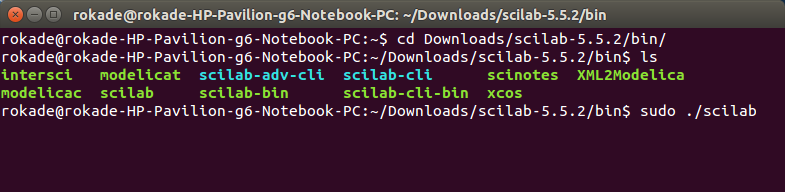
\includegraphics[scale=0.5]{\LocSWfig/linux-cd.png}
      \caption{Linux terminal to launch Scilab}
      \label{linux-cd}
\end{figure}

\subsection{Scilab Arduino toolbox}
Scilab, by default, does not have the capability to connect to
Arduino. All such add-on functionalities are added to \scilab\ using
toolboxes. Just like we have different installation binaries of
\scilab\ for Windows and Linux, we have different toolboxes types for
Windows and Linux. The \scilab\ Arduino toolbox can be found inside
the {\tt Origin/tools/scilab/windows} or {\tt Origin/tools/scilab/linux} directory,
see \fnrefp{fn:file-loc}.  Use the one depending upon
which operating system you are using. The \scilab\ codes for various
experiments mentioned throughout this book can be found in {\tt
            Origin/user-code} directory. The {\tt user-code} directory will have
many sub-directories as per the experiments.

Let us now see how to load the Scilab Arduino toolbox. 
\begin{enumerate}
      \item First launch \scilab. On a Windows system, one may start/launch
            \scilab\ either through the Start menu or by double-clicking on the
            shortcut icon created on the Desktop. On a Linux system, one has to
            start \scilab\ through a terminal with root permissions, as
            explained in section \ref{scilab-installation-linux}.
      \item After launching \scilab, first we have to change the working
            directory. Below the menu bar, locate the tab called {\tt File Browser}. 
            Just below {\tt File Browser}, locate a folder-shaped icon. 
            This icon is used to {\tt Select a directory}. Click on this icon.   
            % click on the {\tt File} menu and then click on
            % the {\tt Change current directory} option as shown in
            % \figref{scilab-cd}.
            % \begin{figure}
            %       \centering
            %       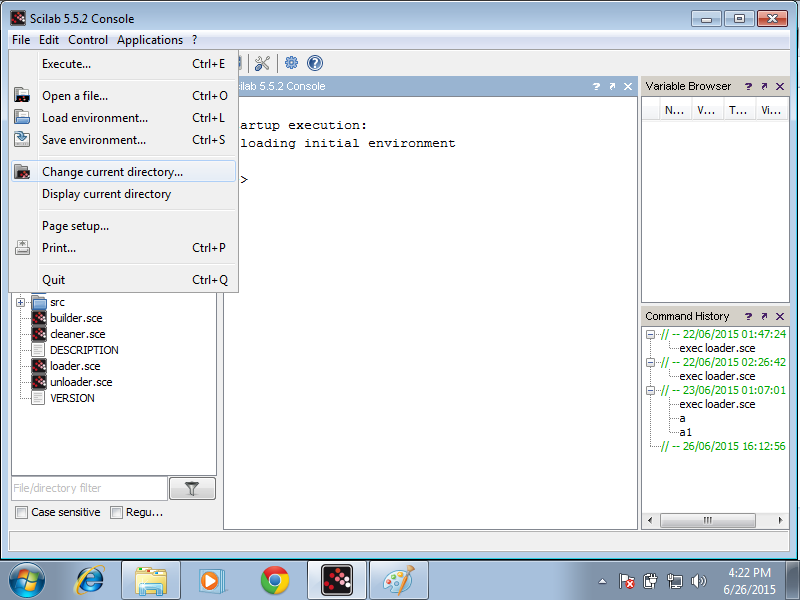
\includegraphics[width=\linewidth]{\LocSWfig/change-directory.png}
            %       \caption{Changing scilab directory}
            %       \label{scilab-cd}
            % \end{figure}
      \item Then, one has to browse to the toolbox folder
                  {\tt Origin/tools/scilab/windows} or {\tt Origin/tools/scilab/linux}, as the case
            may be, and click on, {\tt
                        Open}, as shown in \figref{scilab-browse}.
            \begin{figure}
                  \centering
                  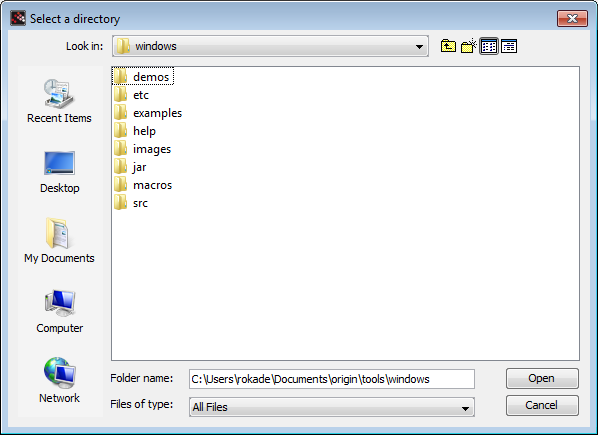
\includegraphics[width=\hgfig]{\LocSWfig/browse-directory.png}
                  \caption{Browsing toolbox directory}
                  \label{scilab-browse}
            \end{figure}
      \item After the previous step, the \scilab\ working directory becomes
            the toolbox folder.  See the {\tt file browser} panel on the
            left-hand side of the \scilab\ console, see \figref{builder}.  It
            will list out the contents of your current working directory. For a
            check, look for the file {\tt builder.sce}.  If you see this file,
            then you are in the right directory.
      \item Next, type the following command on the \scilab\ console: {\tt
            exec builder.sce} - this will build the toolbox and create a file
                  {\tt loader.sce}. This step has to be executed only the first
            time. The output of this step is illustrated in \figref{builder}.
            \begin{figure}
                  \centering
                  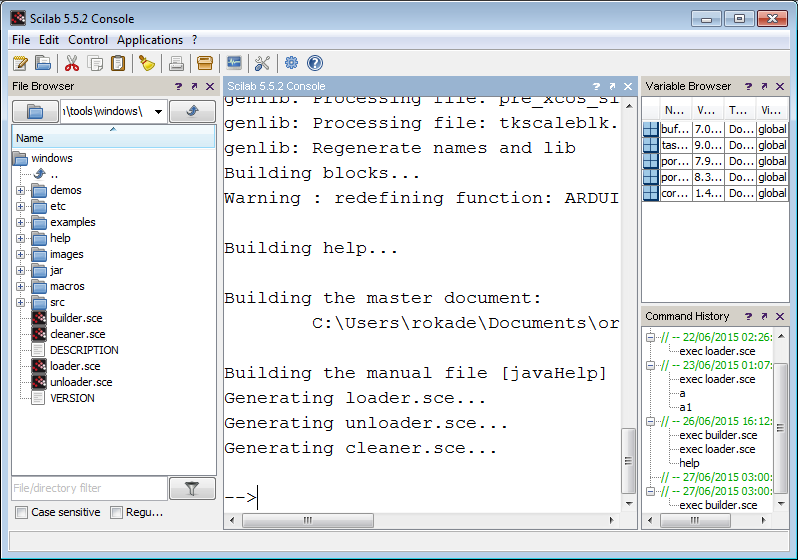
\includegraphics[width=\linewidth]{\LocSWfig/builder.png}
                  \caption{Output of builder.sce}
                  \label{builder}
            \end{figure}
      \item Next, type the command,
            {\tt exec loader.sce} -
            this will load the toolbox. This means all the new functions
            corresponding to the toolbox are loaded in the workspace. It
            will also make available new Xcos blocks, if any.  The
            output of this command is as shown in \figref{loader}.  If you clear
            the workspace for any reason, you will have to execute this command
            once again\footnote{Be careful
                  not to execute the {\tt clear} command.  This will clear the loaded
                  toolbox and you will have to execute the loader.sce file again.}.
            \begin{figure}
                  \centering
                  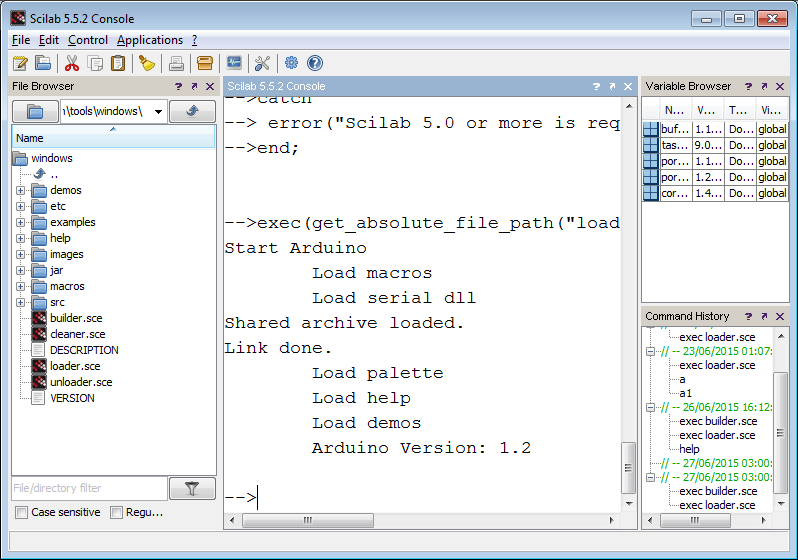
\includegraphics[scale=0.5]{\LocSWfig/loader.png}
                  \caption{Output of loader.sce}
                  \label{loader}
            \end{figure}
\end{enumerate}
The toolbox is now loaded and available for use. 

\subsection{Identifying Arduino communication port number}

Connect \arduino\ board to your computer. On a Windows system, doing
so for the first time will initiate the Windows device identification
routine. It may take a while before it finishes assigning a COM port
number to the \arduino\ board.  If Arduino IDE is installed using the
procedure outlined in \secref{arduino-ide}, required USB drivers for
Arduino get installed automatically.  Hence if you have installed the
Arduino IDE, it should not ask for drivers after you connect it.  As
usually Linux systems come with required drivers, the device is
automatically detected by the OS on connection.

Now let us see how to identify the COM port number. For a Windows
system, open the Device Manager. To do so, right-click on ``My
Computer'' and choose Properties. The Properties window that will open
will have Device Manager in the list on the left-hand side. In the
Device Manager window, look for ``Ports (COM and LPT)''. Double click on
it. It will show you the COM number for \arduino. 

\begin{figure}
      \centering
      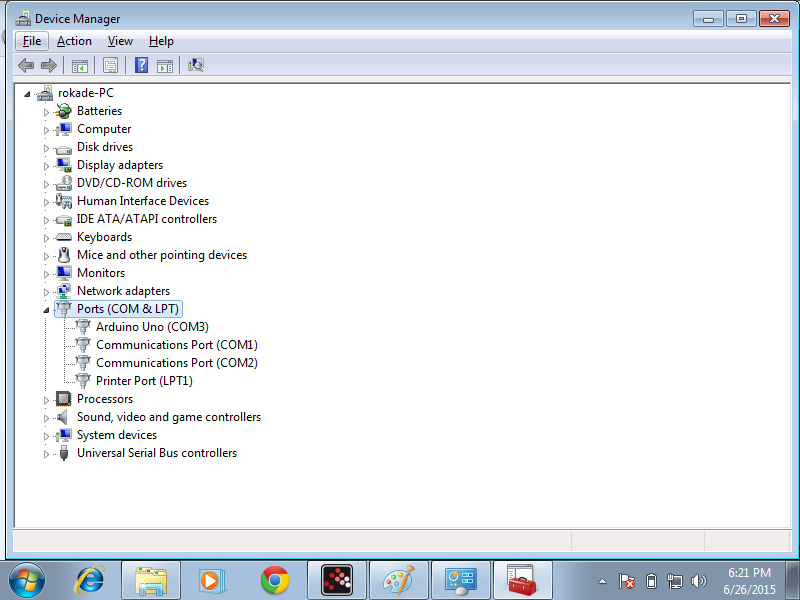
\includegraphics[width=\linewidth]{\LocSWfig/device-manager.png}
      \caption{Device Manager in windows}
      \label{dev-mgr}
\end{figure}

The result of the above exercise is shown in \figref{dev-mgr}.  In
this case, the system has detected Arduino with port number 3, which
appears as COM3.  In this book, we have taken the port for
communication as 2 and written code consistent with this assumption.    
As a result, we will now change it to
COM2\footnote{\label{fn:port}It is possible to leave it at whatever
      port number one gets.  It is also possible to choose any number
      between 2 and 99.  In this case, the port number should be
      changed accordingly in the code.  We will point this out throughout
      the book.}.  To change the port number, double click on the port
number. Its properties window will appear. Click on the ``Port
Settings'' tab and then click on ``Advanced'' button as shown in
\figref{com}.

\begin{figure}
      \centering
      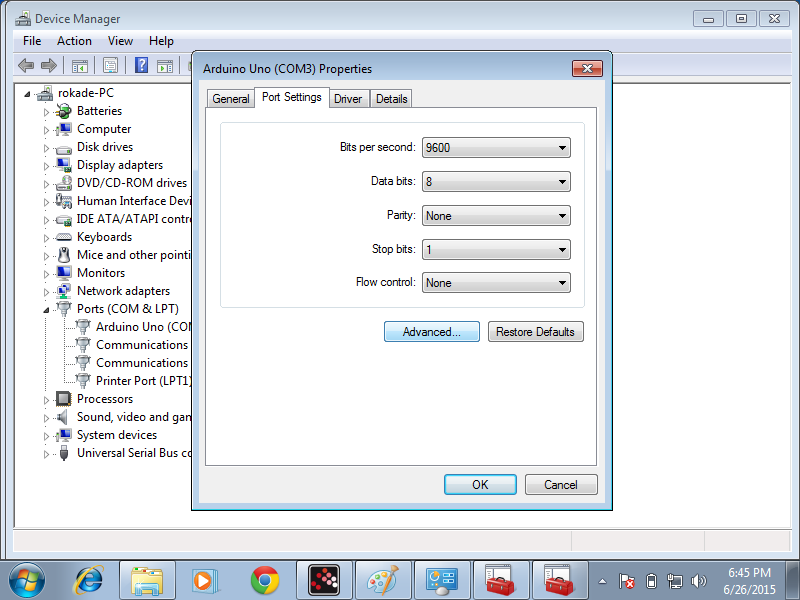
\includegraphics[scale=0.5]{\LocSWfig/com-properties.png}
      \caption{COM port properties window}
      \label{com}
\end{figure}

Click on the drop-down menu for COM port numbers. Choose the port
number COM2.  On clicking on ``OK'', Windows may warn you that the port
number is already in use. But given that you do not have any other USB
device connected you may force change it. Click on ``OK'' to close
all of the device manager windows. Now, we are set to go ahead with
port number 2. The stress on using port number 2 is just to be
consistent throughout the book. It is mainly for a beginner.

Now, let us see how to identify the port number on a Linux
system. Open a terminal by pressing Alt+Ctrl+T keys together. Then
type the following command and press enter, {\tt ls
            /dev/ttyACM*} -
the output of this command is shown in \figref{linux-port}. It has
detected the Arduino with the port number ``ttyACM0''.  The last character
in this string, namely 0, is the port number.  You may get 0 or a
number such as 1 or 2 in your case, for the port number.

\begin{figure}
      \centering
      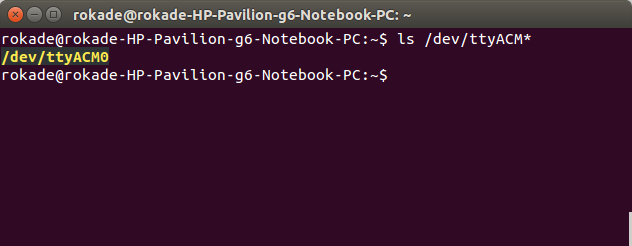
\includegraphics[scale=0.5]{\LocSWfig/linux-port.png}
      \caption{Port number on Linux terminal}
      \label{linux-port}
\end{figure}

\subsection{Testing Scilab-Arduino toolbox}
\label{sec:testing-scilab-arduino}
Now let us test the functioning of the toolbox. 
\begin{enumerate}
      \item Install Arduino IDE, as explained in \secref{sec:ard-start} and
            launch it.
      \item Read into the Arduino IDE, the firmware \ardref{ard:firmware}.
      \item Using the {\tt Upload} option of the Arduino IDE, load this
            firmware on to the \arduino\ board.
      \item Inside the {\tt Origin/tools/scilab} directory, locate a file {\tt
                        test\_firmware.sce}. This file will be used to test whether the
            firmware is properly installed.  This is an important step, as the
            connection between the computer and Arduino breaks down sometimes.
            The Scilab toolbox is unable to identify this difficulty - it has to
            be externally done.  If this difficulty is not identified and
            rectified, one will waste a lot of time and effort trying to debug
            the error.  This test has to be done in case of difficulties.
      \item In the \scilab\ console, type {\tt editor} and press the enter
            key. This will launch the editor. Click on ``File'' menu and choose
            ``Open''. Browse to the directory {\tt Origin/tools/scilab} and choose the
            file {\tt test\_firmware.sce}.  It will open
            \sciref{sci:test-firmware}.  
            %The \scilab\ editor with this file open is as shown in \figref{test-code}.
            %   \begin{figure}
            %     \centering
            %     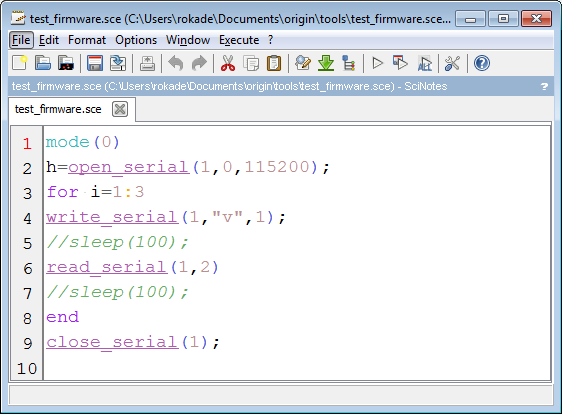
\includegraphics[scale=0.5]{\LocSWfig/test-code.png}
            %     \caption{Scilab code to test toolbox and firmware}
            %     \label{test-code}
            %   \end{figure}
            
      \item If you are using a Windows system and have set your port number
            as COM2, you need not make any changes to the file. Linux users,
            however, will mostly identify the port number as ``ttyACM0''. Hence, 
            they need to change the following line number
            \lstinputlisting[firstline=2,lastline=2]
            {\LocSWchkcode/test_firmware.sce}
            to
            \begin{lstlisting}[style=nonumbers]
  h = open_serial(1,0,115200); 
\end{lstlisting}
            
      \item To execute this code, on the menu bar, click on the {\tt
                        Execute}, option. Then choose {\tt File with no echo}. The output
            will appear on the Console as shown in \figref{test-console}.
            \begin{figure}
                  \centering
                  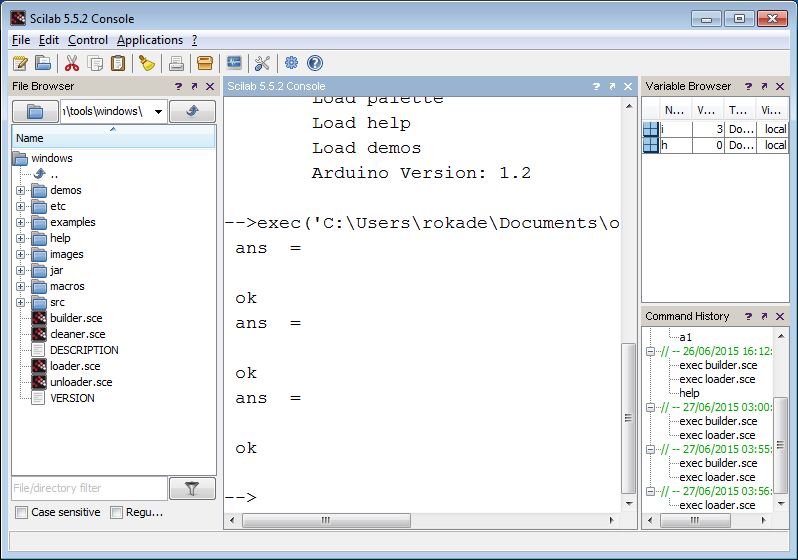
\includegraphics[scale=0.5]{\LocSWfig/test-console.png}
                  \caption{Scilab test code output}
                  \label{test-console}
            \end{figure}
            As shown in the figure, we see the response of this code as ``ans = '' and
            ``ok'' three times.  The
            code basically gives some input to Arduino three times and the
            program inside it returns ``ok'' three times.  This code thus confirms
            the working of the Scilab-Arduino toolbox.  The code also confirms
            that the firmware inside the Arduino is correct.  It is alright if
            one or two of the attempts out of three give a blank response.  But
            all the three responses certainly should not be
            blank\footnote{\label{fn:firmware}If this step is unsuccessful,
                  one should check the connections and re-install the firmware}.
\end{enumerate}

Now let us take a look at the various functions facilitated by the
toolbox. The functions provided in the toolbox are as shown in 
\figref{func}. They are basically categorized into four categories:
configuration, digital, analog and motors. These functions will be
explained in detail in the subsequent chapters as and when they are
used.

\begin{figure}
      \centering
      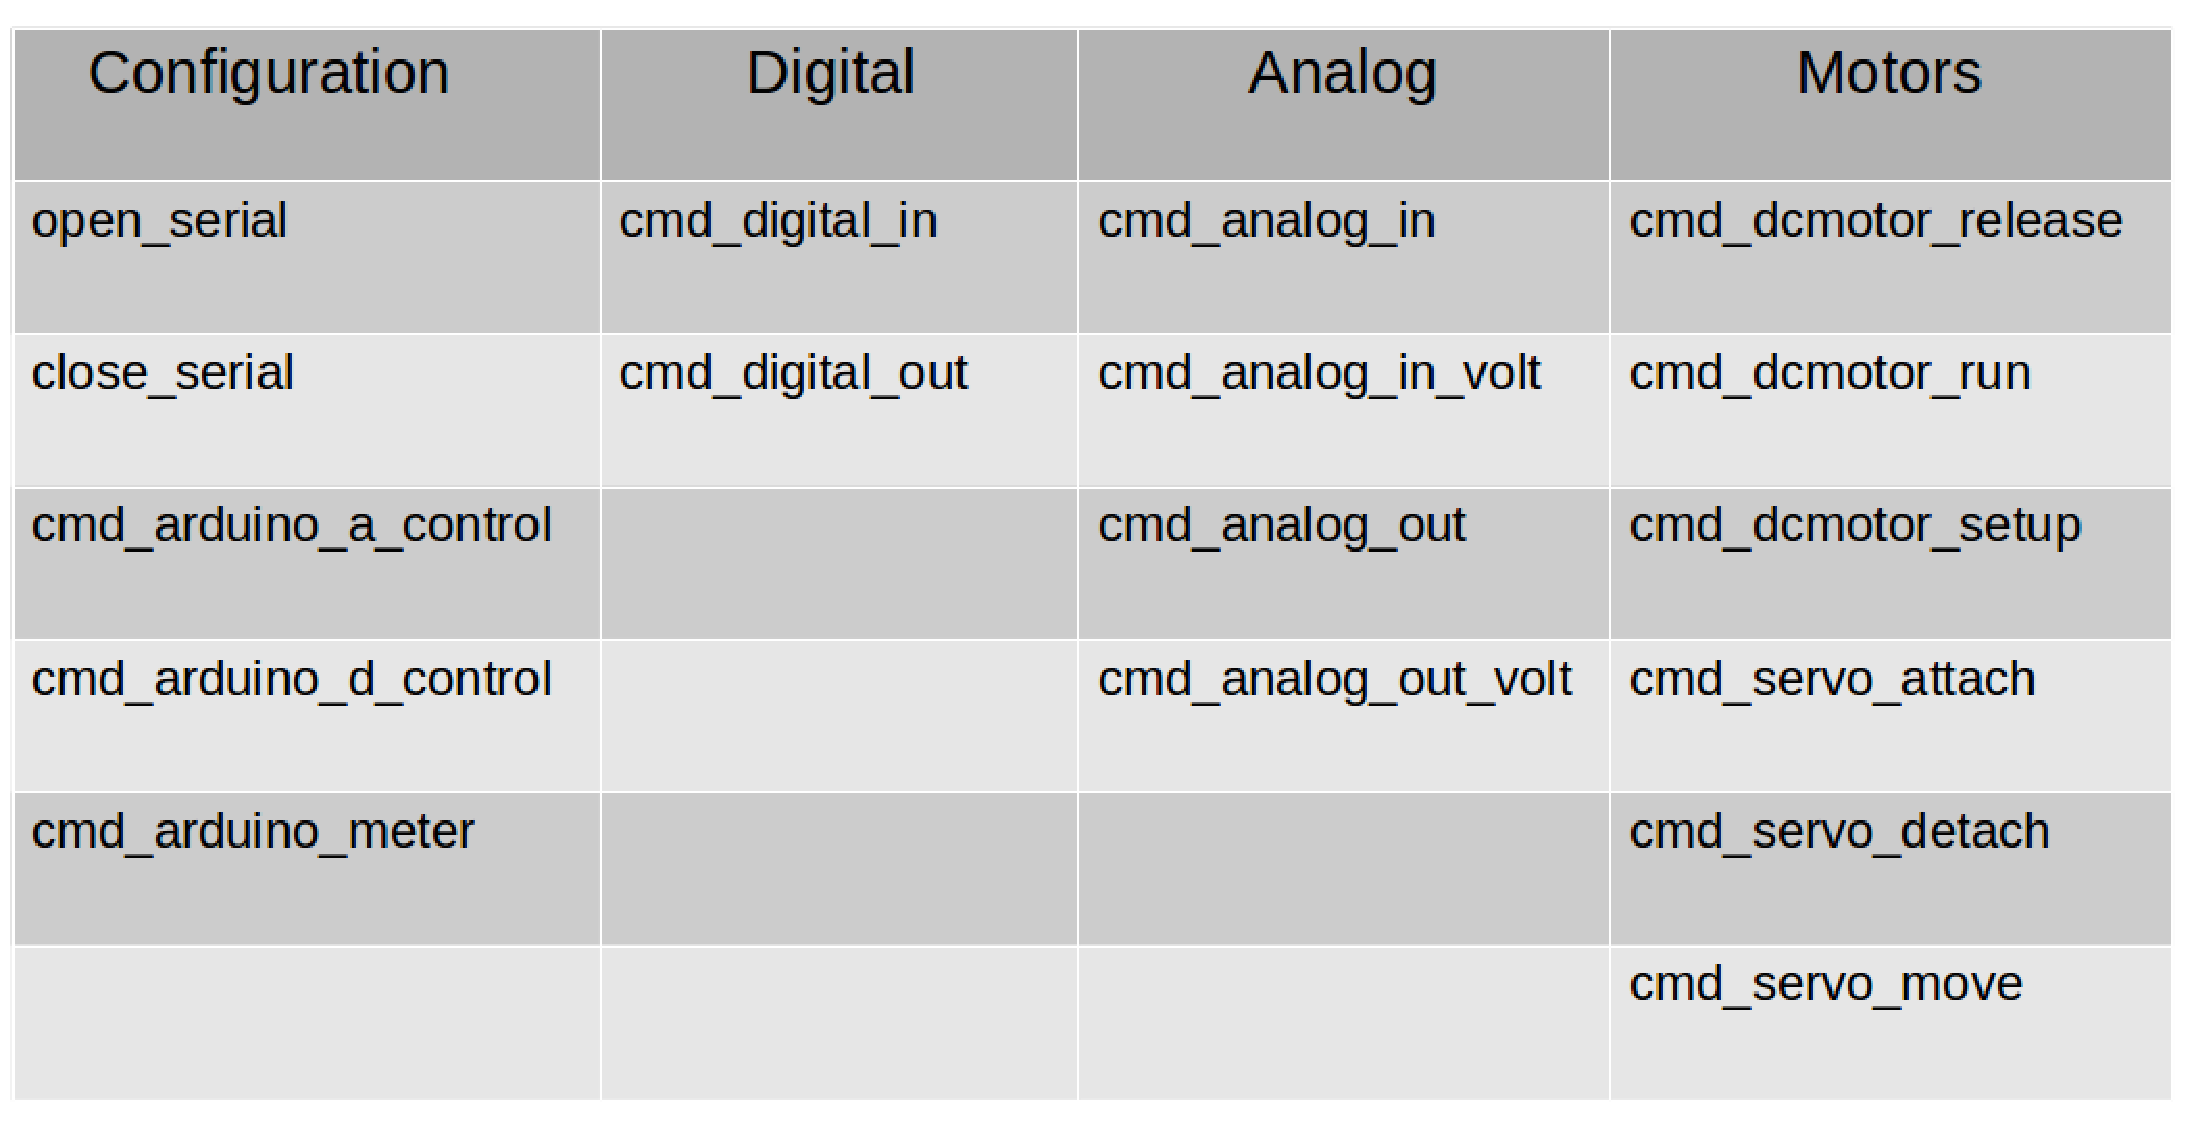
\includegraphics[width=\linewidth]{\LocSWfig/table_functions_crop.pdf}
      \caption{Arduino toolbox functions used in this book}
      \label{func}
\end{figure}

\subsection{Firmware}
\lstset{style=mystyle}
\label{sec:test-firmware-scilab}
\addtocontents{cod}{\protect\addvspace{\codclr}}
We have provided a Scilab code to check whether the firmware has been
properly installed.  That code is listed below.

\begin{scicode}
      \ccaption{A Scilab code to check whether the firmware is
            properly installed or not}{A Scilab code to check whether the
            firmware is properly installed or not.  Available at 
            \LocSWchkbrief{test\_firmware.sce}. Execute this code 
            by following the steps given in section 
            \ref{sec:testing-scilab-arduino}.}
      \label{sci:test-firmware}
      \lstinputlisting{\LocSWchkcode/test_firmware.sce}
\end{scicode}


\section{Xcos}
\label{sec:xcos-start}
Xcos is a graphical editor for \scilab\ \cite{xcos-ref}. Most of the
mathematical manipulations that can be done using \scilab\ scripts,
can be done using Xcos also.  The major advantage of Xcos is the
intuitive interface and easy connectivity across blocks. Xcos even
supports {\tt if else}, {\tt for}, and {\tt while} looping which forms
an integral part of any programming language. It is possible to code
the entire algorithm using Xcos blocks alone. It is also possible to
read from and write to the \scilab\ workspace through Xcos.

\subsection{Downloading, installing and testing}
Xcos comes pre-installed with \scilab. Hence a separate installation
of Xcos is not required. Let us explore the functionalities Xcos has
to offer. Xcos basically provides a graphical interface to \scilab.  

Xcos can be launched from \scilab\ by clicking on the Xcos icon
available on the \scilab\ menu bar. It can also be launched by simply
typing the command {\tt xcos} in the \scilab\ console. When Xcos is
launched, it will open a palette browser.  We have shown this in
\figref{sine-blk}, where we have selected a sine block.  At the time
of launch, Xcos will also open an empty canvas, called an untitled
Xcos window.

\begin{figure}
      \centering
      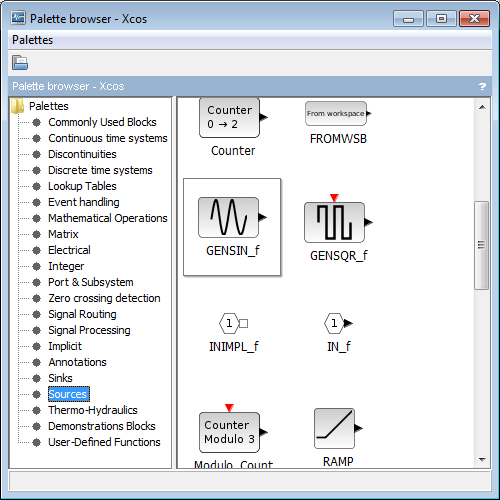
\includegraphics[width=\hgfig]{\LocSWfig/sine-blk.png}
      \caption{Sine generator in palette browser}
      \label{sine-blk}
\end{figure}

% \begin{figure}
% \centering
% 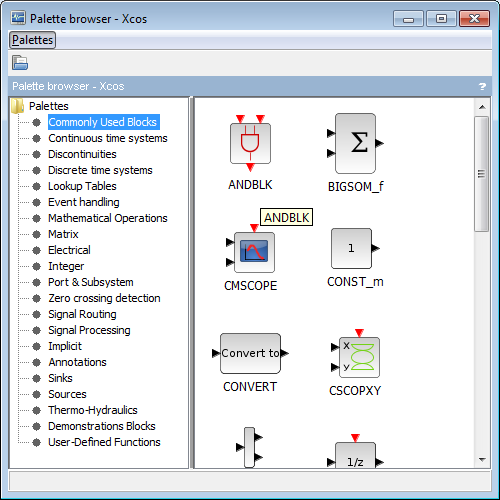
\includegraphics[scale=0.5]{\LocSWfig/palette-browser.png}
% \caption{Palette Browser}
% \label{palette}
% \end{figure}


% \begin{figure}
% \centering
% 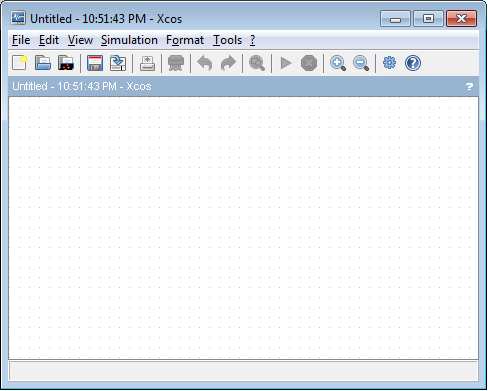
\includegraphics[scale=0.5]{\LocSWfig/untitled-xcos.png}
% \caption{Untitled Xcos window}
% \label{untitled}
% \end{figure}

Palette browser shows all of the available blocks that can be used. It
has been nicely categorized as per the functionality. For example,
blocks that generate signals/values without any input, fall under the
category {\tt Sources}. Similarly, blocks that take signals/values
without giving any output are categorized as {\tt Sinks}. This makes
finding a particular block very easy, specially when one does not know
the name of a block.

The untitled window is the one where one creates the Xcos
code/diagram. The relevant blocks have to be dragged and dropped from
the palette browser to the untitled window. The blocks are then
interconnected and configured as per the simulation, which we will
demonstrate next.

\subsection{Use case}
Let us build a simple Xcos simulation to plot a sine wave. This
simulation requires a sine wave source. It can be found in the {\tt
            Sources} category as shown in \figref{sine-blk}. Drag and drop this
block in the untitled Xcos window. 

Next, we need a block to plot the sine wave. A plotting block can be
found in the {\tt Sinks} category as shown in \figref{plot-blk}. The
name of this block is CSCOPE. Drag and drop this block in the untitled
Xcos window.  On the left-hand side, this block has an input port for
data.  It is black in colour, which may not be obvious in a black and
white printout.  The output from the sine block has to be connected
to this port.  At its top side, the CSCOPE block has another input
port, called an event port.  This is red in colour.  This port is used
to synchronize it with event generating devices.

\begin{figure}
      \centering
      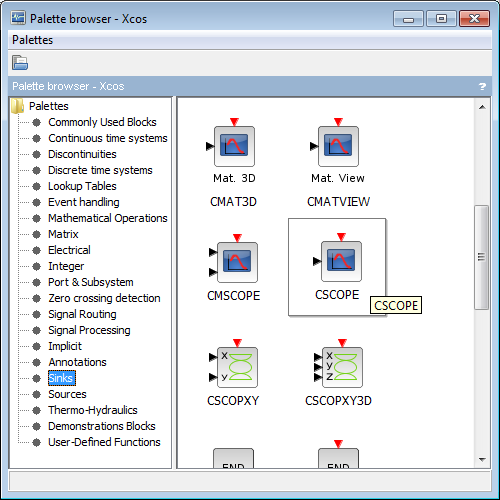
\includegraphics[width=\hgfig]{\LocSWfig/plot-blk.png}
      \caption{CSCOPE block in xcos}
      \label{plot-blk}
\end{figure}

As the CSCOPE block has an
input event port, we need a source that generates events. Hence, the
next block that we need is an event generator block and it can be
found in the {\tt Sources} category. This is illustrated in figure
\ref{clk-blk}. The name of this block is CLOCK\_c. Drag and drop this
block in the untitled Xcos window.

\begin{figure}
      \centering
      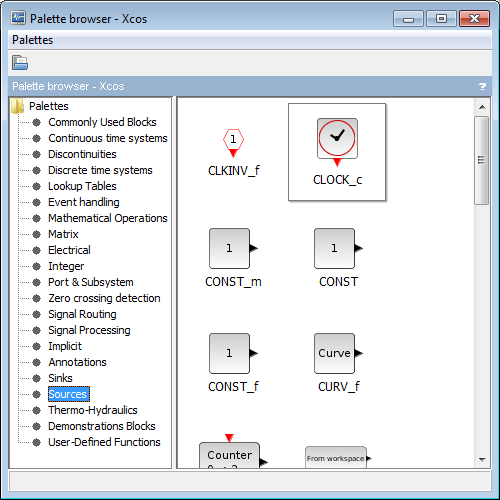
\includegraphics[width=\hgfig]{\LocSWfig/clock-blk.png}
      \caption{CLOCK\_c block in xcos}
      \label{clk-blk}
\end{figure}

The next step is to interconnect the blocks together. A black color
port can only be connected to another black color port. A black color
port cannot be connected to a red color port and vice versa.  That is,
a data port cannot be connected to an event port.  Linking
two blocks is a bit crucial and may need a few attempts before one gets
comfortable. To link two blocks, first click and hold the left mouse
button over the output port of the source block. Without releasing the
mouse button, touch the mouse pointer to the input port of the sink
block. If a connection is possible there, the port will turn
``green''. At this point, release the mouse button and the blocks should
get connected. Follow this procedure and complete the connection as
shown in \figref{sine-gen}.  Save this file with the name {\tt
            sine-generator}.  

\begin{figure}
      \centering
      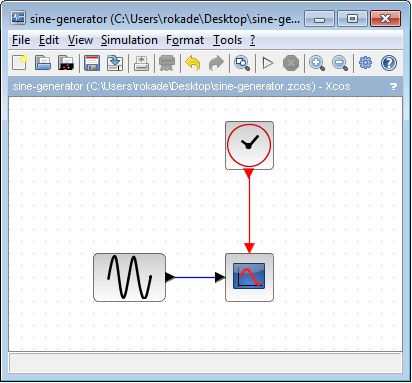
\includegraphics[width=\smfig]{\LocSWfig/sine-gen.png}
      \caption{Sine generator in Xcos}
      \label{sine-gen}
\end{figure}

Let us simulate this Xcos code. On the menu bar, click on the {\tt
            Simulation} menu and choose {\tt Start}. You will get a graphic
window with a running sine wave as shown in \figref{sine-output}.

\begin{figure}
      \centering
      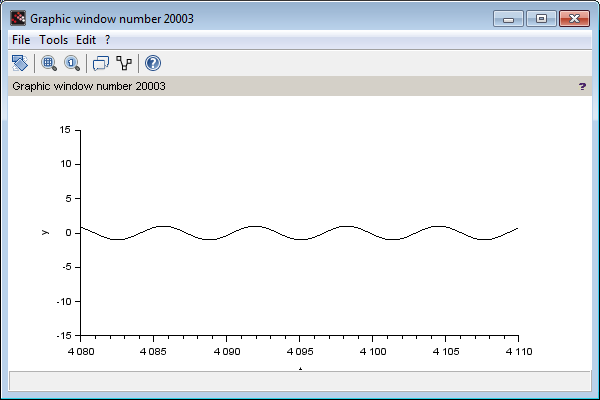
\includegraphics[width=\lgfig]{\LocSWfig/sine-output.png}
      \caption{Sine generator Xcos output}
      \label{sine-output}
\end{figure}

This is because we are running the simulation using the default
configuration.  We would like a stationary plot.  If the simulation is
still running, go to the Simulation menu and choose Stop.  Double
click on the CSCOPE block. Its properties window will appear as shown
in \ref{cscope-config}. Note the value of the {\tt Refresh period}. It
is by default 30. Click on Ok.

\begin{figure}
      \centering
      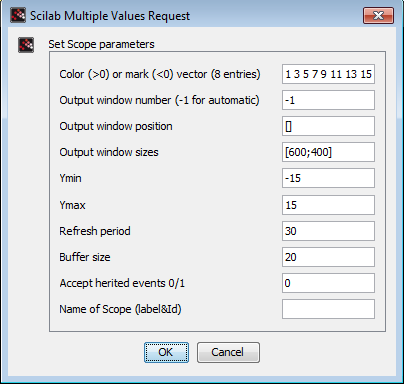
\includegraphics[width=\lgfig]{\LocSWfig/cscope-config.png}
      \caption{CSCOPE configuration window}
      \label{cscope-config}
\end{figure}

Next, on the menu bar, click on the {\tt Simulation} menu and choose
      {\tt Setup}. The {\tt Set Parameters} window will open. The first
parameter is {\tt Final integration time}. It decides for how long the
simulation will run. Change it to be equal to the {\tt Refresh period}
of the CSCOPE block.  That is, change it to 30 as shown in
\figref{sim-setup}. Now start the simulation and you will get a static
plot.  Other paramenters of blocks can also be changed. For example,
one may want to change the input amplitude/frequency or change the
plot scales, etc. All these are left to the reader to explore.

\begin{figure}
      \centering
      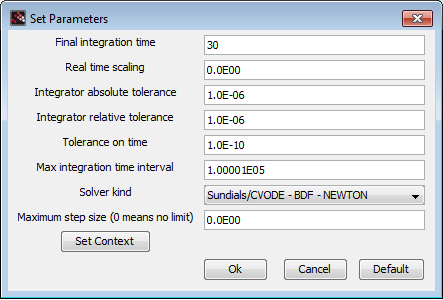
\includegraphics[width=\lgfig]{\LocSWfig/sim-setup.png}
      \caption{Simulation setup window}
      \label{sim-setup}
\end{figure}

Although we have demonstrated a very basic level of Xcos simulation,
this idea can be used for complex processes as well.  Using Xcos, it
is possible to have user-defined blocks. The user can code the
working of the block as a function in \scilab\ script and then call it
from Xcos.  It is also possible to create subsystems.  
One can even read from and write to C binaries.  Xcos comes with
several pre-defined libraries and hence, it is possible to carry out
other kinds of simulation, such as electrical circuit simulation and
basic thermo-hydraulic simulation, for example.  A detailed 
explanation and demonstration are beyond the scope of this book.


\subsection{Xcos-Arduino}
The \scilab\ Arduino toolbox not only provides functions to be used in
\scilab\ scripts but also provides new Arduino-specific blocks. As
shown in \figref{arduino-palette} new Arduino blocks are now available
for use.  Similar to the categorization of the functions, the Xcos
blocks are also categorized as configuration, digital, analog and
motors. Again, it is possible to conduct the experiments only using
Xcos. Xcos codes for every experiment are provided throughout the
book. The Arduino blocks can be easily connected to Xcos native
blocks. A detailed block help for every block can be sought by right-clicking on the block and choosing ``Block help''. This is illustrated
in \figref{blk-help}.

\begin{figure}
      \centering
      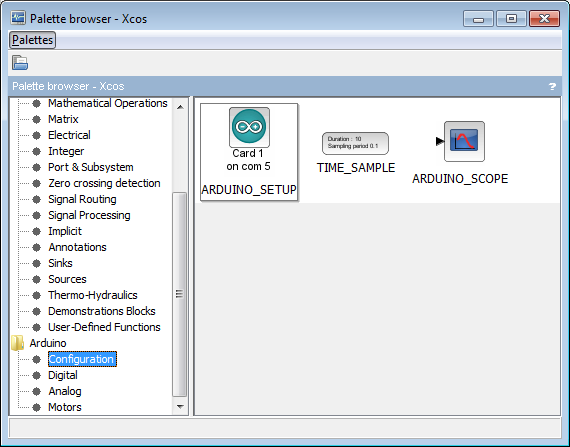
\includegraphics[width=\lgfig]{\LocSWfig/arduino-palette.png}
      \caption{Palette browser showing Arduino blocks}
      \label{arduino-palette}
\end{figure}

\begin{figure}
      \centering
      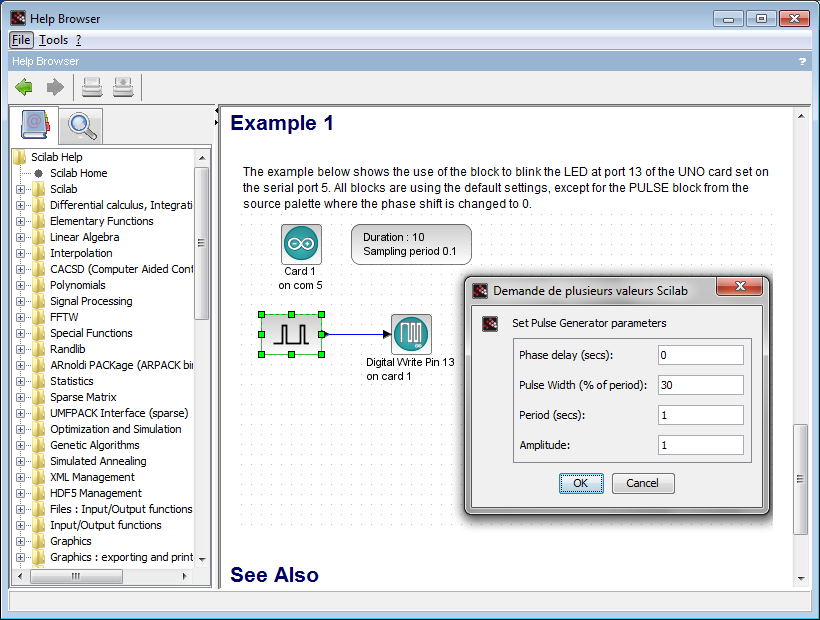
\includegraphics[width=\lgfig]{\LocSWfig/xcos-help.png}
      \caption{Xcos block help}
      \label{blk-help}
\end{figure}

%%%%%python description starts
\section{Python}
\label{sec:python-start}
Python is a general-purpose, high-level, remarkably powerful dynamic programming language 
that is used in a wide variety of application domains. Its high-level built-in data structures, 
combined with dynamic typing and dynamic binding, make it very attractive for Rapid Application Development, 
as well as for use as a scripting or glue language to connect existing components together. 
Python's simple, easy to learn syntax emphasizes readability and therefore reduces the cost of program maintenance. 
Python supports modules and packages, which encourages program modularity and code reuse. 
The Python interpreter and the extensive standard library are available in source or binary form without 
charge for all major platforms, and can be freely distributed \cite{python-ref}.


\subsection{Downloading and installing on Windows} \label{py-windows}
This book uses Python 3 for demonstrating the experiments, both on Windows 
and Linux. Since Python uses indentation to indicate a block of code, 
the users are advised to install a programmer text editor like Atom. 
This editor will allow the readers to modify the Python scripts on their 
machines if they want to. Starting from download, we shall go through the 
steps to set up Python 3 on Windows OS:

\begin{enumerate}
      \item Visit the URL {\tt https://www.python.org/}. 
      At the top of the page, locate the Downloads tab and click on it. 
      At the time of writing this book (as of 21 April 2021), Python 3.9.4 
      is the latest version. Click on Download Python 3.9.4 to download the 
      executable file. The readers may want to download the other versions of 
      Python 3. However, we recommend the installation of Python 3.5 or above. 
      It may be noted that some of the Python 3 versions cannot be used on Windows 7 or earlier.
      \item Locate the executable file and double-click on it to begin the 
      installation. Python 3.9.4 Setup window appears, as shown in \figref{python-windows}. 
      In this window, check the box which says, Add Python 3.9 to PATH and 
      click on Install now.  
      \begin{figure}
            \centering
            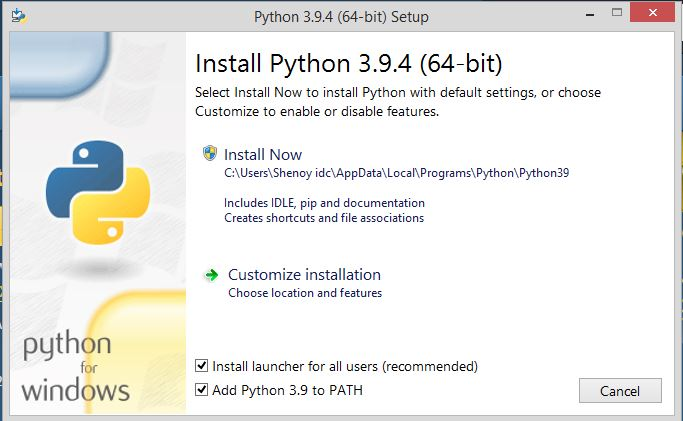
\includegraphics[width=\lgfig]{\LocSWfig/python-windows-install.JPG}
            \caption{Installing Python 3 on Windows}
            \label{python-windows}
      \end{figure}
\end{enumerate}

Once the installation is finished, Python 3.9 App can be launched 
from the Start menu. In this book, we will use the Command Prompt to 
execute the Python scripts. Please note that a Python script has .py as its 
extension. Carry out the steps given below to execute a Python script from 
the Command Prompt:

\begin{enumerate}
      \item Launch the Command Prompt. Press the Windows key+R together. 
      A window, as shown in \figref{windows-run} appears. In the text box adjacent to {\tt Open}, type {\tt cmd}, 
      and press Enter. The Command Prompt, as shown in \figref{windows-cmd} appears. 
      By default, it points to the home directory.  
      \begin{figure}
            \centering
            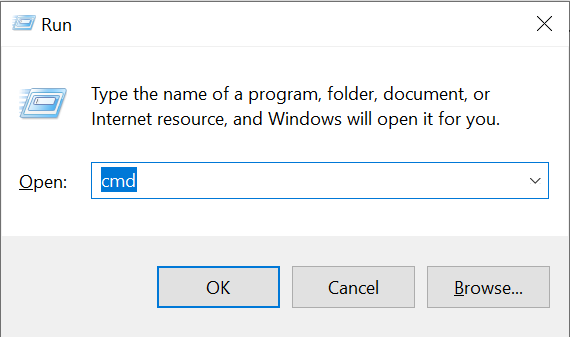
\includegraphics[width=\lgfig]{\LocSWfig/windows-cmd.png}
            \caption{Launching the Command Prompt on Windows}
            \label{windows-run}
      \end{figure}
      \item Now, we will check whether Python 3.9 was installed 
      successfully or not. In the Command Prompt, type {\tt py -{}-version} and 
      press Enter. If this step displays Python 3.9.4 in the following line, 
      the installation was successful. 
      \begin{figure}
            \centering
            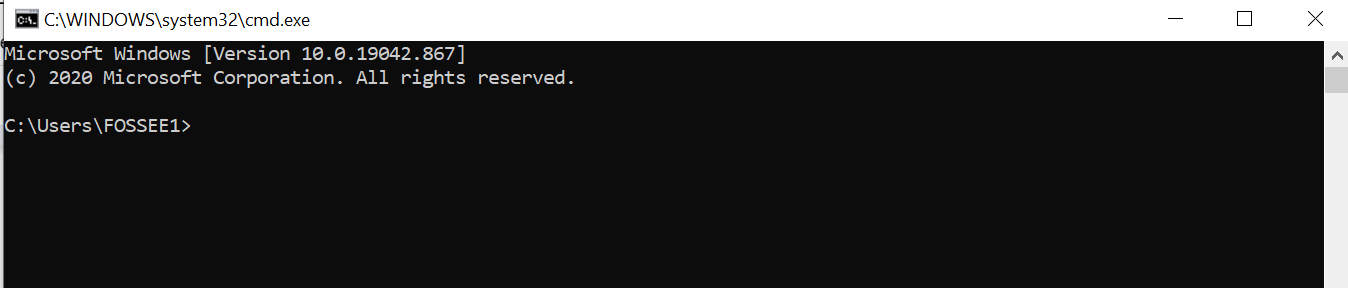
\includegraphics[width=\lgfig]{\LocSWfig/win-command-prompt.png}
            \caption{Command Prompt on Windows}
            \label{windows-cmd}
      \end{figure}
      \item Using the {\tt cd} command, navigate to the directory where your Python 
      script is located. Assuming that your Command Prompt points to the 
      home directory, and you want to navigate to the folder Origin on 
      Desktop, execute the following command: {\tt cd Desktop\textbackslash Origin} \\
      It may be noted that a backslash (\textbackslash) has been used between 
      Desktop and Origin. 
      \item To view the contents of this folder, type {\tt dir} and press Enter.
      \item Suppose you have a Python script named  {\tt FILENAME.py} in this 
      folder. To execute this script, type {\tt python FILENAME.py} and press 
      Enter. The required output will be displayed in the Command Prompt itself. 
      We don’t expect the readers to run the command {\tt python FILENAME.py} at 
      this instant. This command will be helpful while running the Python 
      scripts in the upcoming sections and chapters. 
      \item To exit the Command Prompt, type {\tt exit} and press Enter. 
 
\end{enumerate}

Apart from Python, we need to install Python Serial Port Extension, 
also known as pyserial \cite{pySerial}. To do so, carry out the steps given 
below:
\begin{enumerate}
      \item Launch the Command Prompt, as shown in \figref{windows-run}. 
      \item First, we need to make sure we have pip available. 
      In the Command Prompt, execute the following command: {\tt py -m pip -{}-version} \\ 
      This step should display an output with the version of pip installed. 
      \item Now, install pyserial. In the Command Prompt, execute the following command: 
      {\tt py -m pip install pyserial}  
      \item We will verify whether the pyserial package was installed successfully or not. 
      In the Command Prompt, execute the following command: 
      {\tt pip show pyserial}
      It should show the name, version, etc., of the package. 
      \item To exit the Command Prompt, type {\tt exit} and press Enter. 
\end{enumerate}

\subsection{Downloading and installing on GNU/Linux Ubuntu} \label{py-linux}
On Linux, we can install Python from the terminal. Please ensure that you 
are connected to the Internet. To install Python 3.5, carry out the steps given below:
\begin{enumerate}
      \item Open a terminal by pressing the Alt+Ctrl+T keys together.
      \item Update the system by executing the command {\tt sudo apt-get update}
      \item Install Python3.5 by executing the command given below:\\
      {\tt sudo apt-get install python3.5}
      \item Now, we will check whether Python was installed 
      successfully or not. In the terminal, type {\tt py -{}-version} and 
      press Enter. If this step displays Python 3.8.4 in the following line, 
      the installation was successful. 
\end{enumerate}

Once the installation is finished, Python 3 can be launched 
from the terminal. In this book, we will use the Linux terminal to 
execute the Python scripts. Please note that a Python script has .py as its 
extension. Carry out the steps given below to execute a Python script from 
the terminal:
\begin{enumerate}
      \item Open a terminal by pressing the Alt+Ctrl+T keys together.
      \item Using {\tt cd} command, navigate to the directory where the Python script is located. 
      \item Suppose you have a Python script named  {\tt FILENAME.py}. 
      To execute this script, type {\tt python3 FILENAME.py} and press 
      Enter. The required output will be displayed in the terminal itself. 
      We don’t expect the readers to run the command {\tt python3 FILENAME.py} at 
      this instant. This command will be helpful while running the Python 
      scripts in the upcoming sections and chapters. 
\end{enumerate}

Apart from Python, we need to install Python Serial Port Extension, 
also known as pyserial \cite{pySerial}. To do so, carry out the steps given 
below:
\begin{enumerate}
      \item Open a terminal by pressing the Alt+Ctrl+T keys together.
      \item First, we need to install pip. In the terminal, execute the following command: 
      {\tt sudo apt-get install python3-pip} 
      \item Now, install pyserial. In the terminal, execute the following command:\\ 
      {\tt pip3 install pyserial}  
      \item We will verify whether the pyserial package was installed successfully or not. 
      In the terminal, execute the following command: 
      {\tt pip3 show pyserial}\\
      It should show the name, version, etc., of the package. 
\end{enumerate}

% \begin{enumerate}
%       \item On Ubuntu, Python can be installed from the command line by typing in the
%             following commands:

%             \$ sudo apt-get install python3.5 \\
%             This will install python 3.5 as this set of tools are compatible with python3. It also
%             works all other versions of python3.  
%             \$ pip3 install python-serial \\
%             This will install serial package required for communicating with Arduino Uno.
%       \item 1. On Windows,


%             Download Windows python compiler Self Extracting Archive (.exe)  (32-bit or 64-bit as per your system) from https://www.python.org/downloads/windows/

%             Download Windows pyserial package .exe from https://pypi.python.org/pypi/pyserial/3.4.
%             After downloading run the .exe file and follow the instructions.

%             Now that we have Python installed, open the terminal by typing 'Ctrl+Alt+T'.
%             Enter the command 'python'. This opens the Python REPL (Read Eval Print Loop).
%             Python files have .py extension and .py files can be executed by typing "python3 filename.py"
%             on the python terminal. Please visit the link https://github.com/manasdas17/Python3-Arduino for 
%             the library. 

% \end{enumerate}

\subsection{Python-Arduino toolbox}
\label{sec:python-toolbox}
Python, by default, does not have the capability to connect to Arduino. 
All such add-on functionalities are added to Python using packages. 
The Python-Arduino toolbox can be found inside the {\tt Origin/tools/python} directory, 
see \fnrefp{fn:file-loc}.  This toolbox is compatible for both of the operating systems: Windows and Linux. 
The Python scripts (or codes) for various experiments mentioned throughout this book can be found in 
{\tt Origin/user-code} directory. The {\tt user-code} directory will have many sub-directories as per the experiments. 

In this book, we have created a package named "Arduino" in Python 3.  This package is available at 
{\tt Origin/tools/python}. This package makes use of the functions available in pyserial \cite{pySerial} to 
establish serial communication with Arduino. In this package, we have added functions required to run 
various experiments on \arduino. Using this basic set of functions, the user can define other functions to operate
upon the Arduino. Please note that the "Arduino" package and the Arduino firmware  given 
in \ardref{ard:firmware} are required to run the experiments. 

Now, we will see how to import (or load) the "Arduino" package inside a Python script to run 
various experiments provided in this book. In a Python script, add {\tt from Arduino.Arduino import Arduino} 
at the top of the script. When we add {\tt from Arduino.Arduino import Arduino} in a script, the function "from" 
searches for "Arduino" only in that directory where our script is saved. That's why all the scripts in Python 
must be saved in a folder that contains the "Arduino" package. In this book, "Arduino" package has been saved 
in the folder where the Python scripts for each chapter are available. For the sake of convenience, we have 
added {\tt from Arduino.Arduino import Arduino} in all the Python scripts provided in this book. 
To run a particular experiment, one can follow the steps as given in \secref{py-windows} or \secref{py-linux}. 


\subsection{Firmware}
\lstset{style=mystyle}
\label{sec:test-firmware-python}
\addtocontents{pyd}{\protect\addvspace{\codclr}}
We have provided a Python code to check whether the firmware has been properly installed. That code is listed below.  
Please ensure that you have uploaded the Arduino firmware given in \ardref{ard:firmware} on the \arduino\ board.

\begin{pycode}
      \pcaption{A Python script to check whether the firmware is properly installed
            or not}{A Python script to check whether the firmware is properly installed
            or not.  Available at 
            \LocFIMpybrief{test\_firmware.py}. 
            Execute this script by following the steps given in \secref{py-windows} or \secref{py-linux}. If the execution is
            successful, you should expect three "ok" messages.}
      \label{py:test-firmware}
      \lstinputlisting{\LocFIMpycode/test_firmware.py}
\end{pycode}



%%%%%python description ends

%%%%%%Julia descrition starts

\section{Julia} \label{sec:julia-start}
Julia is a high-level, high-performance dynamic programming language for 
technical computing, with a syntax familiar to users of other technical computing 
environments \cite{julia-ref}. While it is a general-purpose language and can be used to write any 
application, many of its features are well suited for numerical analysis and 
computational science. Julia provides a sophisticated compiler, distributed 
parallel execution, numerical accuracy, and an extensive mathematical function
library. 

% This is a set of tools that provide functionality in Julia, to program the \arduino. 

\subsection{Downloading and installing on Windows} \label{julia-install-windows}
This book uses Julia 1.6.0 for demonstrating the experiments, both on Windows and Linux. 
Julia does not use indentation to indicate a block of code, unlike Python. However, 
the users are advised to install a programmer text editor like Atom. This editor will 
allow the readers to modify the Julia source files on their machines if they want to. 
Alternatively, one can also use Notepad (on Windows) or gedit (on Linux Ubuntu) to edit 
Julia source files. Starting from download, we shall go through the steps to set 
up Julia 1.6.0 on Windows OS:
\begin{enumerate}
      \item Visit the URL {\tt https://julialang.org/}.  At the top of the page, 
      locate the Download tab and click on it. From the Current stable release, 
      download the required Julia binaries (32 or 64-bit) for Windows, as shown in \figref{julia-download}. 
      At the time of writing this book, the Current stable release refers to Julia 1.6.0 
      as of March 24, 2021, as shown in \figref{julia-download}. In this book, we will perform 
      experiments with a 64-bit installation of Julia 1.6.0.
      \item Locate the executable file. Right-click on it and hit 
      Run as administrator to begin the installation. After selecting the Installation Directory, 
      a window named Select Additional Tasks appears as shown in \figref{julia-windows-install}. 
      In this window, check the box which says, Add Julia to PATH and click on Next to continue the installation. 
\end{enumerate}

\begin{figure}
      \centering
      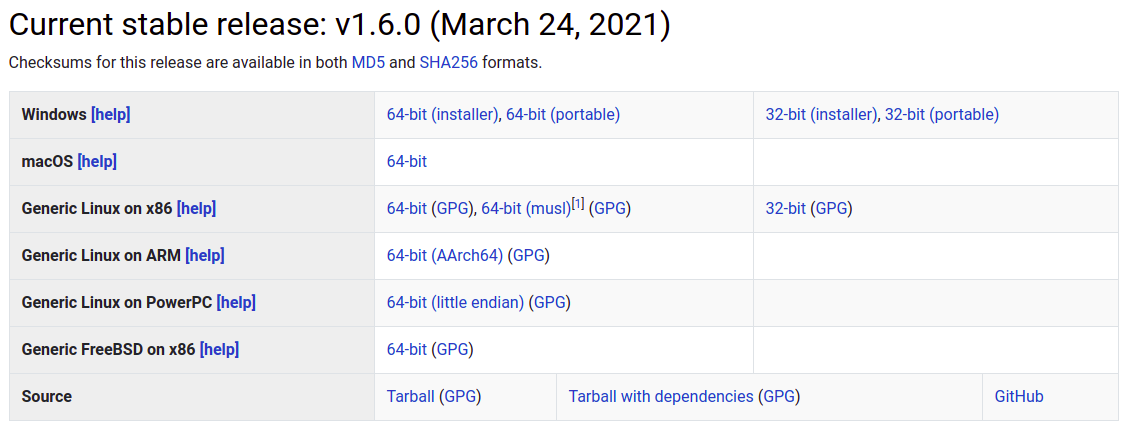
\includegraphics[width=\textwidth]{\LocSWfig/julia-download.png}
      \caption{Julia's website to download 64-bit Windows/Linux binaries}
      \label{julia-download}
\end{figure}

\begin{figure}
      \centering
      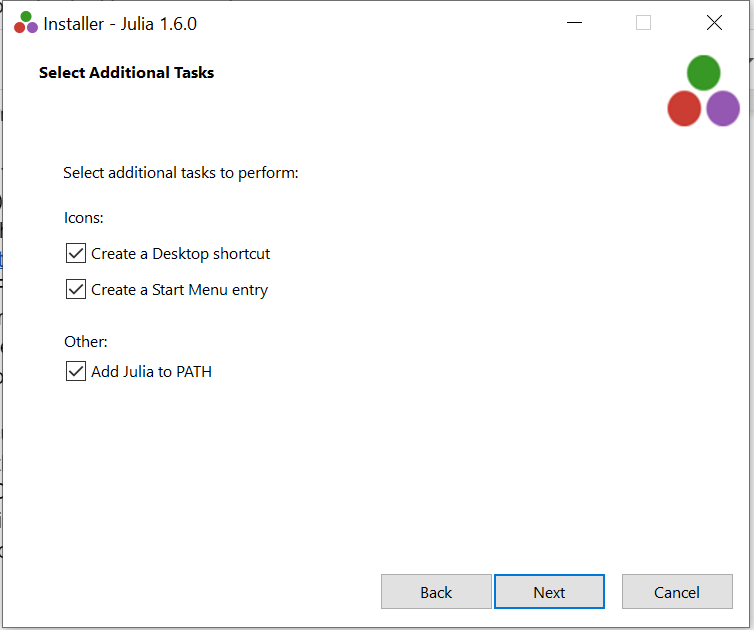
\includegraphics[width=\lgfig]{\LocSWfig/julia-windows-install.png}
      \caption{Installing Julia 1.6.0 on Windows}
      \label{julia-windows-install}
\end{figure}

Once the installation is finished, Julia 1.6.0 App can be launched either 
from the Start menu or from the Command Prompt. In this book, we will use the Command 
Prompt to execute the Julia source files. Please note that a Julia source file has .jl as its extension. 
Carry out the steps given below to execute a Julia source file from the Command Prompt:
\begin{enumerate}
      \item Launch the Command Prompt. Press the Windows key+R together. A window, as shown in \figref{windows-run} 
      appears. In the text box adjacent to Open, type cmd, and press Enter. The Command Prompt, as shown in
       \figref{windows-cmd} appears. By default, it points to the home directory.
      \item Now, we will check whether Julia 1.6.0 was installed successfully or not. 
      In the Command Prompt, type {\tt julia -{}-version} and press Enter. 
      If this step displays julia version 1.6.0 in the following line, the installation was successful.
      \item Using the {\tt cd} command, navigate to the directory where your Julia source file is located. 
      Assuming that your Command Prompt points to the 
      home directory, and you want to navigate to the folder Origin on 
      Desktop, execute the following command: {\tt cd Desktop\textbackslash Origin} \\
      It may be noted that a backslash (\textbackslash) has been used between 
      Desktop and Origin. 
      \item To view the contents of this folder, type {\tt dir} and press Enter.
      \item Suppose you have a Julia source file named {\tt FILENAME.jl} in this 
      folder. To execute this script, type {\tt julia FILENAME.jl} and press 
      Enter. The required output will be displayed in the Command Prompt itself. 
      We don't expect the readers to run the command {\tt julia FILENAME.jl} at 
      this instant. This command will be helpful while running the Python 
      scripts in the upcoming sections and chapters. 
      \item To exit the Command Prompt, type {\tt exit} and press Enter. 
\end{enumerate}

Apart from Julia, we need to install the SerialPorts \cite{julia-serial-ports} package in Julia. This package will be
required to establish serial communication with Arduino boards. Please make sure that 
you are connected to the Internet. To install the package, we will use {\tt Pkg}. 
It is Julia's built-in package manager and handles operations such as installing, 
updating and removing packages in Julia. To install the SerialPorts package, carry out the steps given below:
\begin{enumerate}
      \item Launch the Command Prompt, as shown in \figref{windows-run}.
      \item In the Command Prompt, type {\tt julia} and press Enter. It should launch Julia in an interactive session (also known as a read-eval-print loop or "REPL"), as shown 
      in \figref{julia-repl-windows}. When run in interactive mode, Julia displays a banner and 
      prompts the user for input. By default, Julia REPL appears in Julian prompt. It is the default mode of 
      operation; each new line initially starts with {\tt julia>}, as 
      shown in \figref{julia-repl-windows}. It is here that you can enter Julia expressions. 
      Hitting return or Enter after a complete expression has been entered will evaluate 
      the entry and show the result of the last expression. 
      \begin{figure}
            \centering
            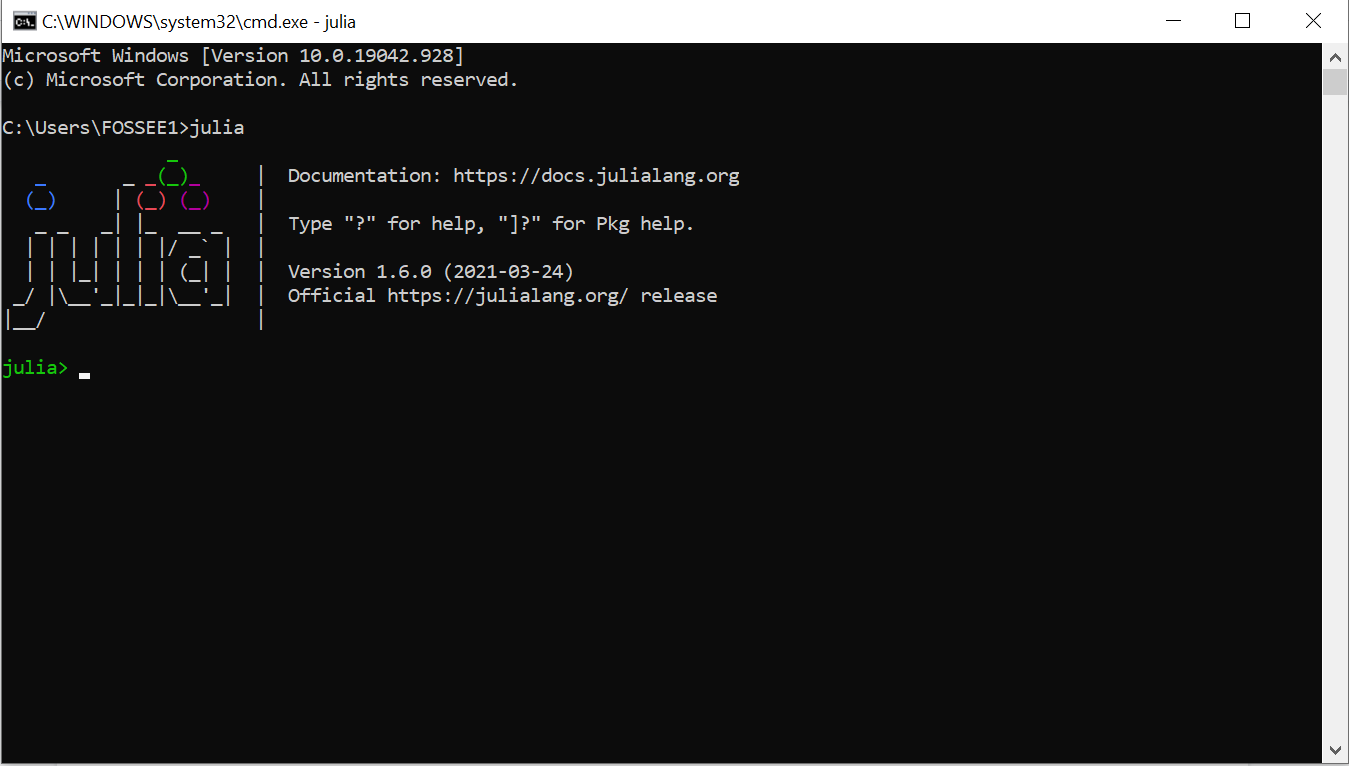
\includegraphics[width=\textwidth]{\LocSWfig/julia-repl-windows.png}
            \caption{Windows command prompt to launch Julia REPL}
            \label{julia-repl-windows}
      \end{figure}
      \item Now, we need to enter the {\tt Pkg} REPL in Julia. From the Julia REPL, 
      press {\tt ]} to enter the {\tt Pkg} REPL. The moment you press 
      {\tt ]}, you enter {\tt Pkg} REPL, as shown in \figref{julia-pkg-windows}.
      \begin{figure}
            \centering
            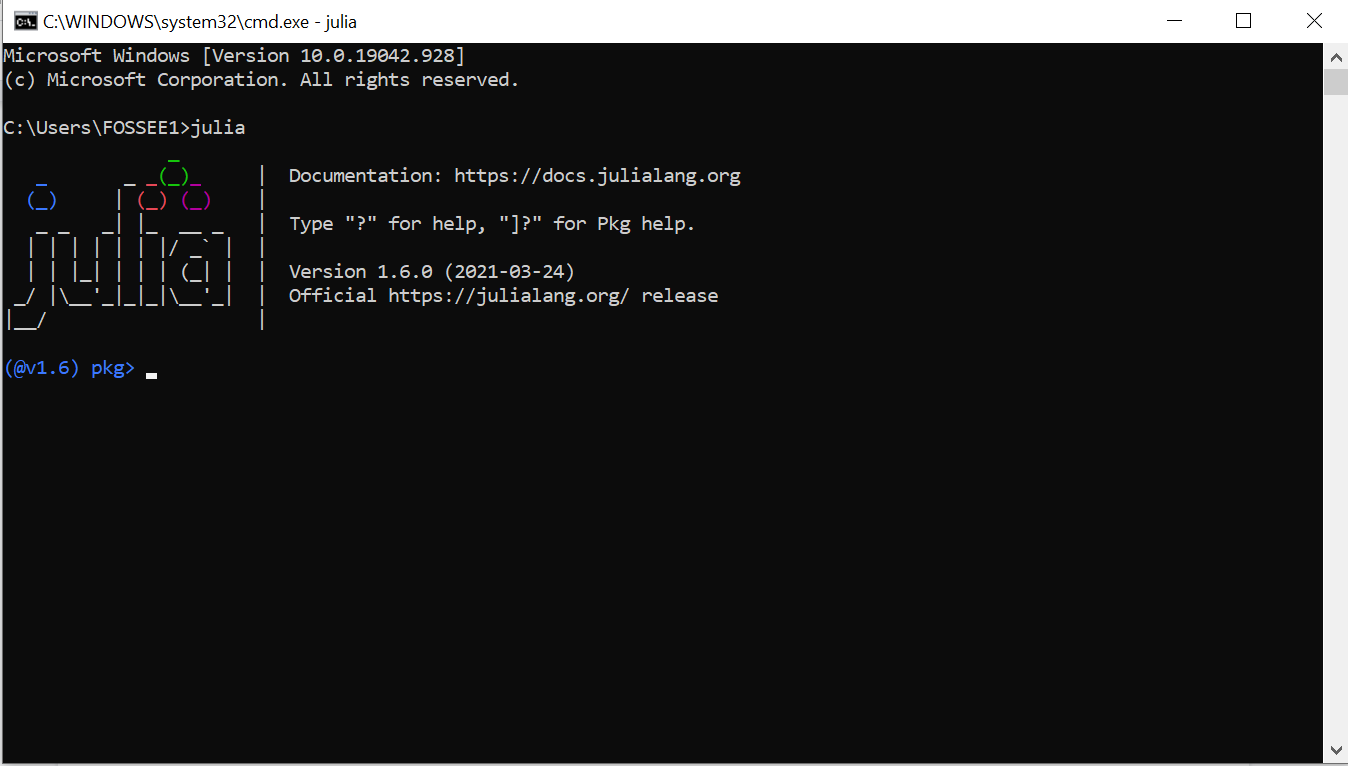
\includegraphics[width=\textwidth]{\LocSWfig/julia-pkg-windows.png}
            \caption{Windows command prompt to enter Pkg REPL in Julia}
            \label{julia-pkg-windows}
      \end{figure}
      \item In {\tt Pkg} REPL, type {\tt add SerialPorts} and press Enter. It might take a few seconds/minutes  
      to get this package installed. Once it is installed, {\tt Pkg} REPL should show a message,
      like "3 dependencies successfully precompiled in 9 seconds (4 already precompiled)."
\end{enumerate}

We can also check the status of this package to verify whether it has been installed 
successfully or not. For this, we need to get back to Julia REPL. Inside {\tt Pkg}
REPL, press backspace. The moment you press backspace, you get back to Julia REPL, as shown in 
\figref{julia-repl-windows}. Now, type {\tt using Pkg} and press Enter. This command will not 
generate any output. Now type {\tt Pkg.status()} and press Enter. It should display the 
list of packages installed in Julia's environment. Please make sure that SerialPorts 
is present in the list of packages being shown. To exit the interactive session, type CTRL+D or type {\tt exit()}. 

\subsection{Downloading and installing GNU/Linux Ubuntu} \label{julia-install-linux}
We will now explain the installation of Julia on the GNU/Linux operating system. 
We shall perform the installation on the 64-bit Ubuntu 18.04 LTS operating system.  
These instructions will work for other GNU distributions, too, with little or 
no modification. This book uses Julia 1.6.0. To install it, carry out the steps
given below: 
\begin{enumerate}
      \item First, update your system. Open the Terminal. Type
                  {\tt sudo apt-get update} and press Enter. 
      \item Find out your operating system support for 64-bit
            instructions. Open the Terminal. Type {\tt uname -m} and press Enter. If it returns ``x86\_64'', then your computer has 64-bit
            operating system. 
      \item Visit the URL {\tt https://julialang.org/}.  At the top of the page, 
      locate the Download tab and click on it. From the Current stable release, download the 
            required Linux binaries (32 or 64-bit) for Generic Linux on x86, as shown in \figref{julia-download}.  
            At the time of writing this book, the Current stable release refers to Julia 1.6.0 as of March 24, 2021, 
            as shown in  \figref{julia-download}. In this book, we will perform experiments with a 64-bit installation of Julia  v1.6.0. 
      \item Locate the executable (tar.gz) file. Assuming that you have downloaded the tar file in {\tt Downloads} directory, perform the following
            steps on the Terminal:
            \begin{quote}
                  {\tt cd {\large\textasciitilde}/Downloads\\
                        tar -xvzf julia-1.6.0-linux-x86\_64.tar.gz\\
                        sudo cp -r julia-1.6.0 /opt/}
            \end{quote}
      \item Finally, create a symbolic link to {\tt julia} inside the
            {\tt /usr/local/bin} folder. In the same Terminal session from the previous step, issue the 
            following command: \\
            {\tt sudo ln -s /opt/julia-1.6.0/bin/julia /usr/local/bin/julia} 
\end{enumerate}

Julia is now installed and can be invoked from the Terminal. There are two modes in which Julia 
source files can be executed: Interactive mode and Non-interactive mode. In this book, 
we will execute source files in the latter mode i.e., from the Terminal. The readers are encouraged to explore
the former mode on their own. Please note that a Julia source file has .jl
as its extension. Carry out the steps given below to execute a Julia source file from
the Terminal: 
\begin{enumerate}
      \item Open a Terminal by pressing Ctrl+Alt+T keys together.
      \item Now, we will check whether Julia 1.6.0 was installed successfully or not. 
      In the Terminal, type {\tt julia -{}-version} and press Enter. 
      If this step displays {\tt julia version 1.6.0} in the following line, the installation was successful.
      \item Using the {\tt cd} command, navigate to the directory where your Julia source file is located. 
      Assuming that your Terminal points to the 
      home directory, and you want to navigate to the folder Origin on 
      Desktop, execute the following command: {\tt cd Desktop/Origin/}
      \item Suppose you have a Julia source file named {\tt FILENAME.jl} in this 
      folder. To execute this script, type {\tt julia FILENAME.jl} and press 
      Enter. The required output will be displayed in the Terminal itself. 
      We don't expect the readers to run the command {\tt julia FILENAME.jl} at 
      this instant. This command will be helpful while running the Python 
      scripts in the upcoming sections and chapters. 
\end{enumerate}

\begin{figure}
      \centering
      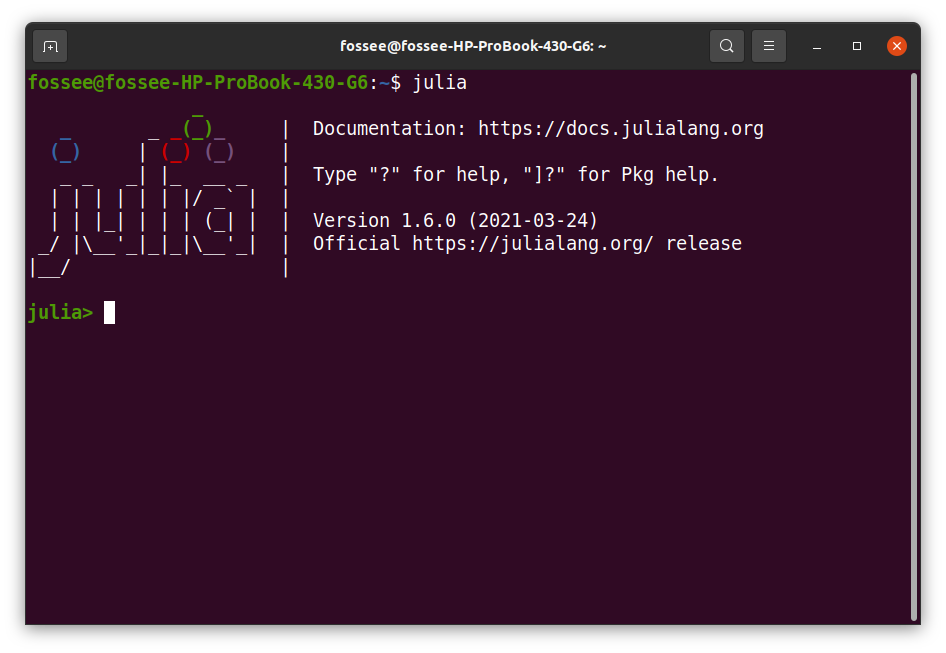
\includegraphics[width=\textwidth]{\LocSWfig/julia-terminal-repl.png}
      \caption{Linux terminal to launch Julia REPL}
      \label{julia-repl}
\end{figure}


Now, we will install a package named SerialPorts \cite{julia-serial-ports}. This package will be required to 
establish serial communication with Arduino boards. Please ensure that you 
are connected to the Internet. To install the package,  
we will use {\tt Pkg}. It is Julia's built-in package manager and 
handles operations such as installing, updating, and removing packages in Julia. 
For installing LibSerialPort, carry out the steps given below:
\begin{enumerate}
      \item Open a Terminal by pressing Ctrl+Alt+T keys together. Type {\tt julia} and press Enter.
      It should launch Julia in an interactive session (also known as a read-eval-print loop or "REPL"), as shown 
      in \figref{julia-repl}. When run in interactive mode, Julia displays a banner and 
      prompts the user for input. By default, Julia REPL appears in Julian prompt. It is the default mode of 
      operation; each new line initially starts with {\tt julia>}, as 
      shown in \figref{julia-repl}. It is here that you can enter Julia expressions. 
      Hitting return or Enter after a complete expression has been entered will evaluate 
      the entry and show the result of the last expression.  
      \item From the Julia REPL, press {\tt ]} to enter the {\tt Pkg} REPL. The moment you press 
            {\tt ]}, you enter {\tt Pkg} REPL, as shown in \figref{julia-pkg}. 
      \item In {\tt Pkg} REPL, type {\tt add SerialPorts} and press Enter. It might take a few seconds  
            to get this package installed. Once it is installed, {\tt Pkg} REPL should show a message,
            like "5 dependencies successfully precompiled in 12 seconds." 
\end{enumerate}

\begin{figure}
      \centering
      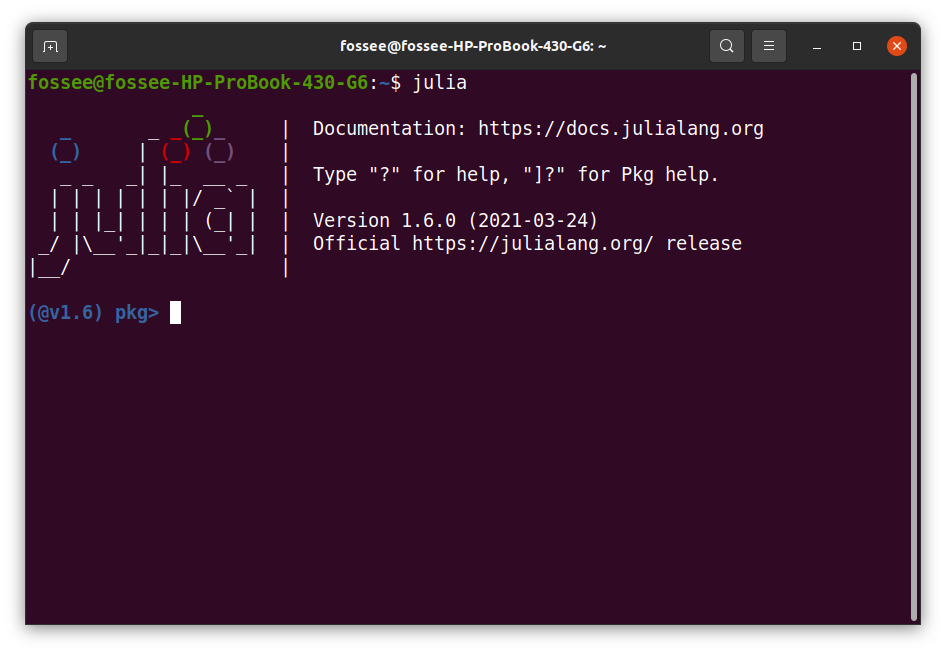
\includegraphics[width=\textwidth]{\LocSWfig/julia-pkg.png}
      \caption{Linux terminal to enter Pkg REPL in Julia}
      \label{julia-pkg}
\end{figure}

We can also check the status of this package to verify whether it has been installed 
successfully or not. For this, we need to get back to Julia REPL. Inside {\tt Pkg}
REPL, press backspace. The moment you press backspace, you get back to Julia REPL, as shown in 
\figref{julia-repl}. Now, type {\tt using Pkg} and press Enter. This command will not 
generate any output. Now type {\tt Pkg.status()} and press Enter. It should display the 
list of packages installed in Julia's environment. Please make sure that SerialPorts 
is present in the list of packages being shown. To exit the interactive session, type CTRL+D or type {\tt exit()}. 


\subsection{Julia-Arduino toolbox}
\label{sec:julia-toolbox}
Julia, by default, does not have the capability to connect to Arduino. 
All such add-on functionalities are added to Julia using toolboxes. 
The Julia-Arduino toolbox can be found inside the {\tt Origin/tools/julia} directory, 
see \fnrefp{fn:file-loc}.  This toolbox is compatible for both of the operating systems: Windows and Linux. 
The Julia source files (or codes) for various experiments mentioned throughout this book can be found in 
{\tt Origin/user-code} directory. The {\tt user-code} directory will have many sub-directories as per the experiments. 

In this book, we have created a module named "ArduinoTools" in Julia.  This module is available at 
{\tt Origin/tools/julia}. This module makes use of the functions available in the SerialPorts package to 
establish serial communication with Arduino. In this module, we have added functions required to run 
various experiments on \arduino. Using this basic set of functions, the user can define other functions to operate
upon the Arduino. 

% Please note that the module "ArduinoTools" and the Arduino firmware  given in \ardref{ard:firmware} are required to run the experiments. 

Now, we will see how to import (or load) the module named "ArduinoTools.jl" inside a Julia source file to run 
various experiments provided in this book. In a Julia source file, add {\tt include("ArduinoTools.jl")} at the top of the file. 
When we add {\tt include("ArduinoTools.jl")} in a source file, the function "include" searches for "ArduinoTools.jl" 
only in that directory where our source file is saved. That's why all the source files in Julia 
must be saved in a folder that contains the file "ArduinoTools.jl." In this book, "ArduinoTools.jl" has been saved 
in the folder where the Julia source files for each chapter are available. For the sake of convenience, we have 
added {\tt include("ArduinoTools.jl")} in all the Julia source files provided in this book. 
To run a particular experiment, one can follow the steps as given in \secref{julia-install-windows} and \secref{julia-install-linux}. 

\subsection{Firmware}
\lstset{style=mystyle}
\label{sec:test-firmware-julia}
\addtocontents{cod}{\protect\addvspace{\codclr}}
We have provided a Julia source file (code) to check whether the firmware has been
properly installed.  That file is listed below.  Please ensure that 
you have uploaded the Arduino firmware given in \ardref{ard:firmware} on \arduino.

\begin{juliacode}
      \jcaption{A Julia source file to check whether the firmware is properly installed
            or not}{A Julia source file (code) to check whether the firmware is properly installed
            or not.  Available at
            \LocFIMjuliabrief{test\_firmware.jl}. Execute this source file by following the steps 
            given in \secref{julia-install-windows} and \secref{julia-install-linux}. If the execution is
            successful, you should expect three "ok" messages. }
      \label{julia:test-firmware}
      \lstinputlisting{\LocFIMjuliacode/test_firmware.jl}
\end{juliacode}




%%%%%%%%OpenModelica description starts


\section{OpenModelica}
\label{sec:OpenModelica-start}
OpenModelica is a free and open-source environment based on the Modelica modeling language 
for simulating, optimizing, and analyzing complex dynamic systems \cite{om-ref}.
It is a powerful tool that can be used to design and simulate complete control systems. 
% The toolbox 'OpenModelica-Arduino' enables the interfacing of Arduino with OpenModelica by calling a set of c functions from OpenModelica.   

In the upcoming sections, we have provided the steps to install OpenModelica on Windows and Linux. 
After installing OpenModelica, the readers should watch the tutorials on OpenModelica provided on 
{\tt https://spoken-tutorial.org/}. Ideally, one should go through all the tutorials labeled as Basic. 
However, we strongly recommend the readers should watch the second and third tutorials, i.e., 
{\tt Introduction to OMEdit} and {\tt Examples through OMEdit}.


\subsection{Downloading and installing on Windows} \label{openmodelica-install-windows}
This book uses Stable Development of OpenModelica 1.17.0 for demonstrating 
the experiments, both on Windows and Linux. It may be noted that 
OpenModelica requires approximately 8 GB of space for its installation. 
Starting from download, we shall go through the steps to set up OpenModelica 
1.17.0 on Windows OS:

\begin{enumerate}
      \item Visit the URL {\tt https://openmodelica.org/}.  At the top of the page, locate the Download tab. On hovering the cursor on this tab, a drop-down menu appears. In that menu, click on Windows. 
      \item From the section Download Windows, click on the binaries 1.17.0 (32bit/64bit) next to the Stable Development of OpenModelica. 
      \item A webpage named Index of /omc/builds/windows/releases/1.17/0 appears. Now, click on 32-bit or 64-bit depending on your operating system. We will continue with a 64-bit installation. 
      \item Once you select 64-bit, a webpage named Index of /omc/builds/windows/releases/1.17/0/64bit appears. You should get a list of files here. Click on the executable (.exe) file to download the binaries for OpenModelica.
      \item Locate the executable file and double-click on it to begin the 
      installation. After double-clicking on the executable file, 
      you might get an alert on your screen (something like Windows protected your PC). 
      If this happens, locate More info in this alert window and click on 
      Run Anyway, as shown in \figref{om-run-anyway} to continue with the 
      installation. All the default parameters of the installation are acceptable. 
\end{enumerate}

\begin{figure}
      \centering
      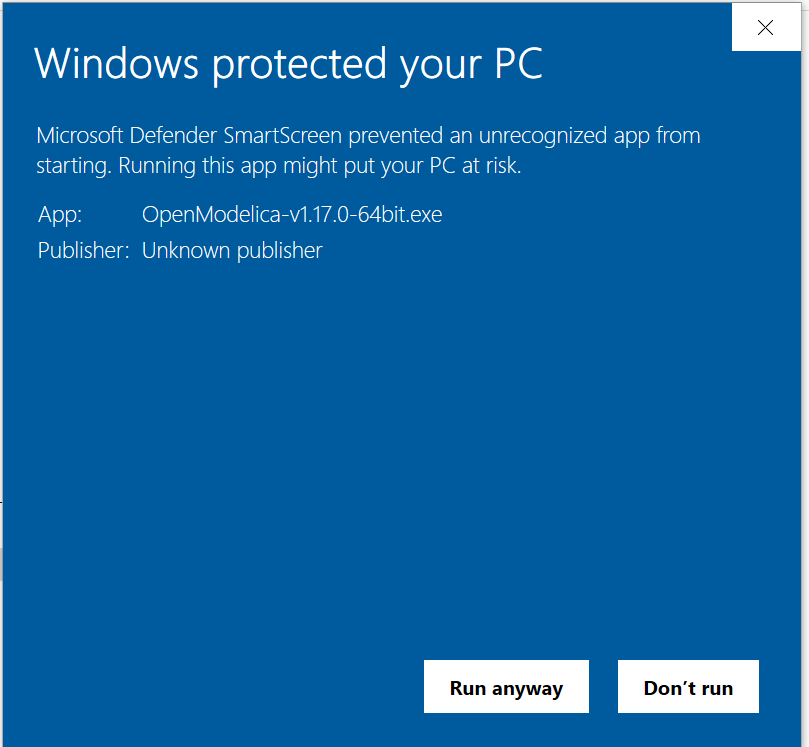
\includegraphics[width=\lgfig]{\LocSWfig/openmodelica-run-anyway.png}
      \caption{Allowing Microsoft Defender to run the executable file}
      \label{om-run-anyway}
\end{figure}

Once OpenModelica has been installed, OpenModelica Connection Editor (OMEdit) 
can be launched from the Start menu.  When you 
launch OMEdit for the first time, you might get a notification for setting up 
Modelica Standard Library version, as shown in \figref{om-help}. Here, you 
should choose the option "Load MSL v3.2.3" and click OK.  To know how to execute models 
in OMEdit, the readers are advised to refer to \secref{OpenModelica-code-execution}. 


\subsection{Downloading and installing on GNU/Linux Ubuntu} \label{openmodelica-install-linux}
On Linux, we can install OpenModelica from the terminal. The readers are advised to visit 
{\tt https://openmodelica.org/download/download-linux} and follow the instructions for installing OpenModelica.
We recommend the readers should install the latest stable version of OpenModelica. 
Once OpenModelica has been installed successfully, OpenModelica Connection Editor (OMEdit) can be launched
from the terminal. Open a terminal by pressing Alt+Ctrl+T and type OMEdit. When you 
launch OMEdit for the first time, you might get a notification for setting up 
Modelica Standard Library version, as shown in \figref{om-help}. Here, you 
should choose the option "Load MSL v3.2.3" and click OK.  
\begin{figure}
      \centering
      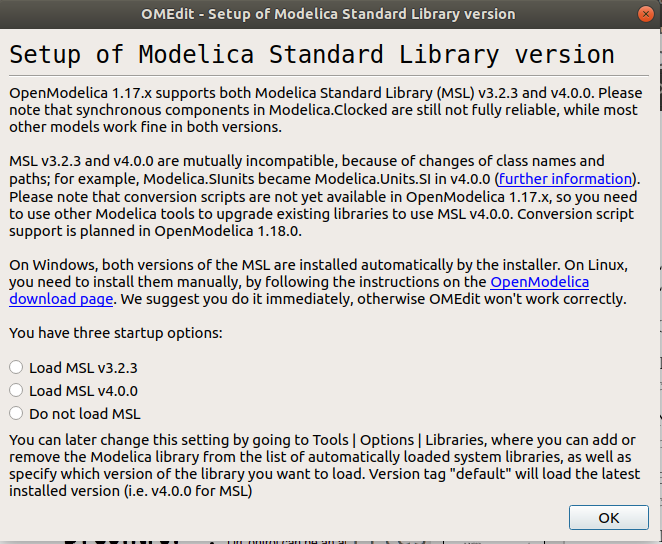
\includegraphics[scale=0.55]{\LocSWfig/OMEdit-libraries.png}
      \caption{Setup of Modelica Standard Library version}
      \label{om-help}
\end{figure}
To know how to execute models in OMEdit, the readers are advised to refer to \secref{OpenModelica-code-execution}. 

\subsection{Simulating models in OpenModelica}\label{OpenModelica-code-execution}
Once you launch OMEdit (either on Windows or on Linux Ubuntu), you should expect a user interface, 
as shown in \figref{om-ui}. In the bottom right of \figref{om-ui}, we can 
see that there are four different tabs - Welcome, Modeling, Plotting, and 
Debugging. In the language of OpenModelica, we refer to these tabs as Perspectives. 
By default, OMEdit gets launched in the Welcome Perspective. We now briefly describe each 
of these Perspectives, as given below:
\begin{enumerate}
      \item Welcome Perspective: It shows the list of recent files and the list of the 
      latest news from {\tt https://www.openmodelica.org}.
      \item Modeling Perpective: It provides the interface where users can 
      create and design their models.
      \item Plotting Perspective: It shows the simulation results of the models. 
      Plotting Perspective will automatically become active 
      when the simulation of the model is finished successfully.
      \item Debugging Perspective: The application automatically switches to Debugging Perspective 
      when the user simulates the class with an algorithmic debugger \cite{om-ref}.
\end{enumerate}

In the left of \figref{om-ui}, there is Libraries Browser below which you can view
the list of libraries loaded in your current session of OMEdit. By default, OMEdit 
comes with a few default libraries, like Modelica, ModelicaReference, etc., as shown in
\figref{om-ui}. These default libraries might not be visible if you have not set up the
Modelica Standard Library version, as given in \figref{om-help}. 
\begin{figure}
      \centering
      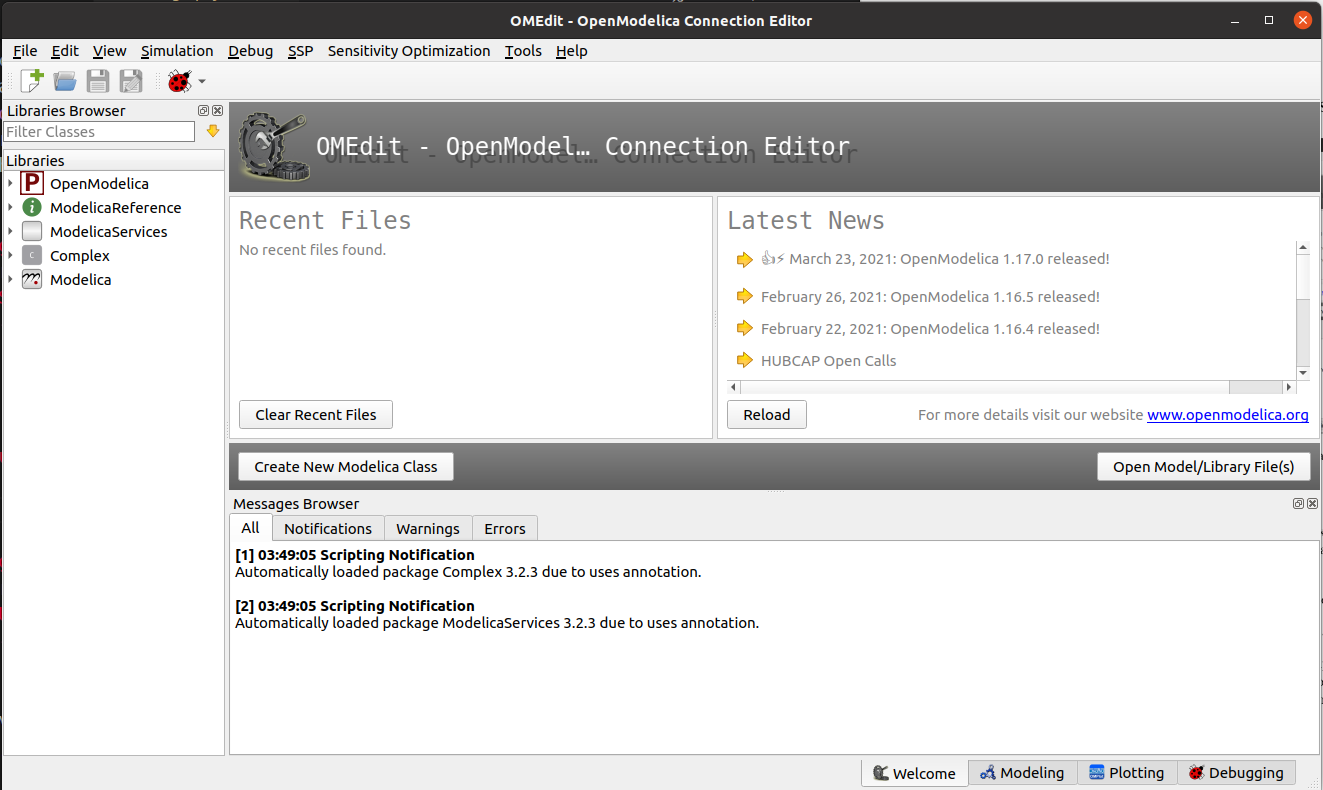
\includegraphics[width=\textwidth]{\LocSWfig/OMEdit-UI.png}
      \caption{User Interface of OMEdit}
      \label{om-ui}
\end{figure}

The files or models in OpenModelica have `.mo' extensions. Though there are several ways to simulate or run 
an OpenModelica model, we will execute the models by utilizing the user interface of OMEdit. To open 
a model in OMEdit, go to the menu bar of OMEdit and click on File -> Open Model/Library File(s), as shown 
in \figref{om-model-open}. Then, select the desired model (with `.mo' extension) and click Open. The names of tabs in
this book have been mentioned according to OpenModelica 1.17.0. You might observe a bit
of difference in these names while working with other versions of OpenModelica. 

\begin{figure}
      \centering
      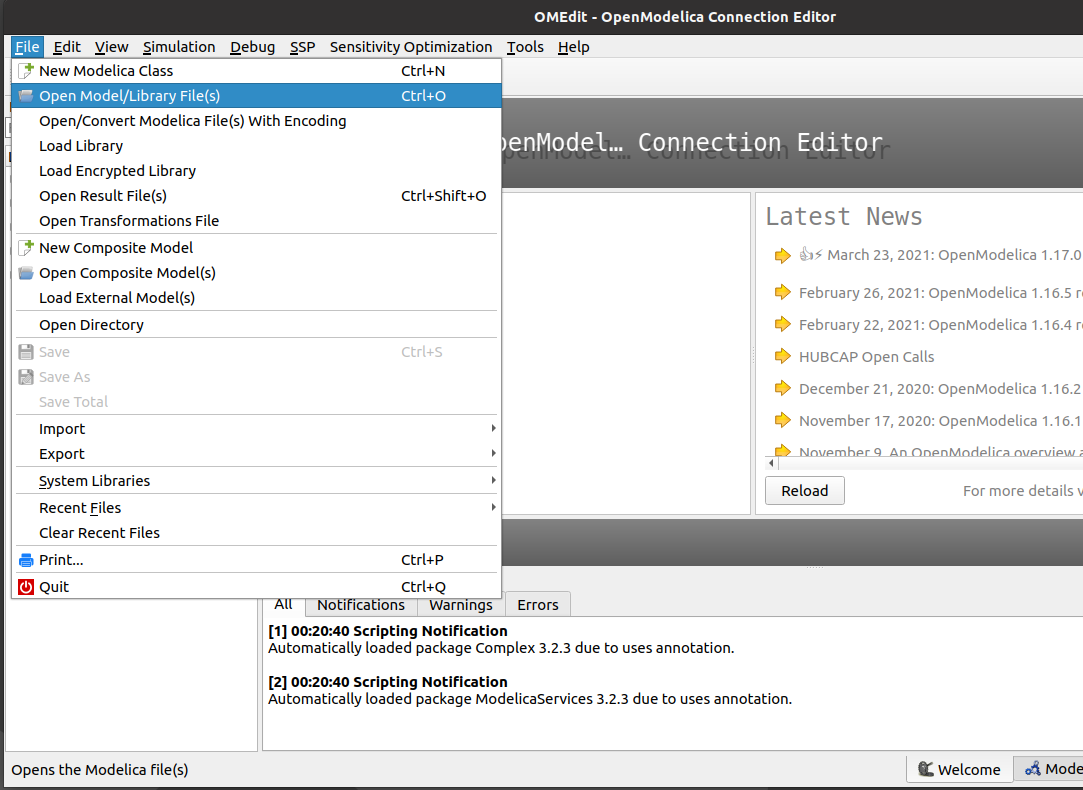
\includegraphics[width=\textwidth]{\LocSWfig/om-open-model.png}
      \caption{Opening a model in OMEdit}
      \label{om-model-open}
\end{figure}

\begin{figure}
      \centering
      \includegraphics[width=\textwidth]{\LocSWfig/om-Modeling.png}
      \caption{Opening a model in diagram view in OMEdit}
      \label{om-modeling}
\end{figure}


\begin{figure}
      \centering
      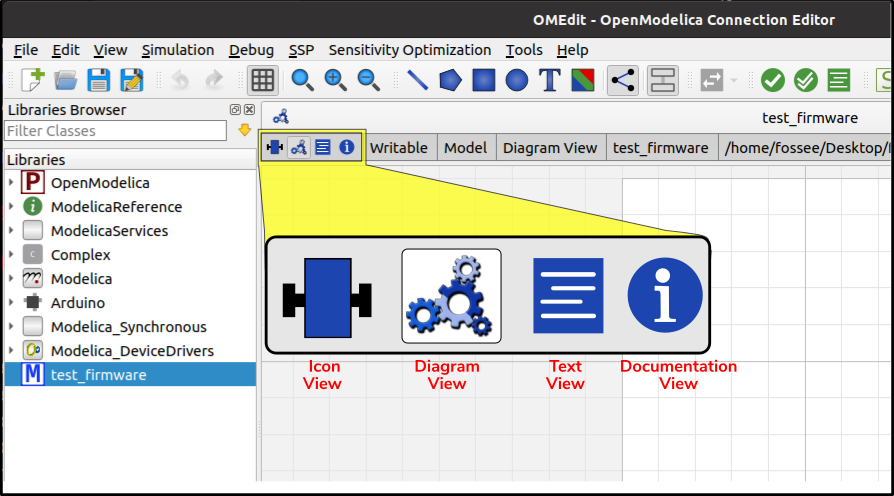
\includegraphics[width=\textwidth]{\LocSWfig/om-modeling-views.png}
      \caption{Different views of a model in OMEdit}
      \label{om-views}
\end{figure}


\begin{figure}
      \centering
      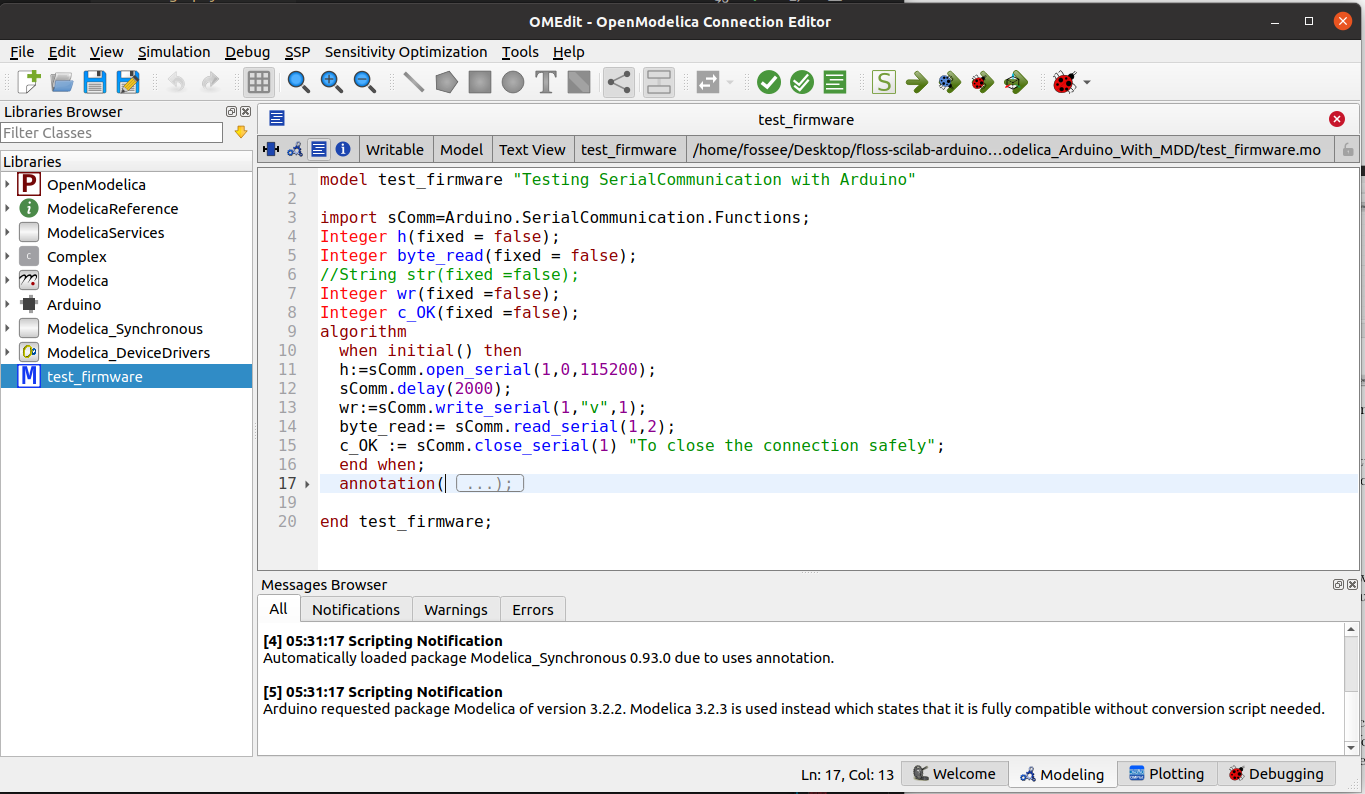
\includegraphics[width=\textwidth]{\LocSWfig/om-text-view.png}
      \caption{Opening a model in text view in OMEdit}
      \label{om-text-view}
\end{figure}

Once you have opened the model in OMEdit, that model should appear under the Libraries
browser, as shown in \figref{om-ui}. To view or simulate that model, you need to 
double-click on the model. It will open the model in Modeling perspective with a Diagram View, as shown 
in the \figref{om-modeling}. In this perspective, there are four different views of 
a model: Icon View, Diagram View, Text View, and Documentation View. All these views have been highlighted in \figref{om-views}. 
By default, OMEdit opens any model in Diagram View. Hence, the models 
having code in text format won't be visible by default in Modeling 
Perspective. To see the code in text format, we need to open the model in 
Text View. For our experiments, we will use Text view mainly. To view the code written for this model, 
we need to click on Text View, as shown in \figref{om-views}. In Text view, the code is now visible, as 
shown in \figref{om-text-view}. Now, one can modify the model as per the requirements. 

Now, we will see how to simulate this model. For this, we need to ensure that OMEdit 
is in Modeling Perspective. Next, we will click on the green right-sided arrow, named as 
Simulate, as shown in \figref{om-simulate}. When we click on Simulate, OMEdit will first 
compile the model and then, it will simulate the model for the time specified in the model itself. 
As OMEdit provides an elegant user interface for simulating the models, 
it will open an output window the moment you click on Simulate. \figref{om-sim-success}
shows the output window after the simulation of our model is finished. Also, we can
observe that the OMEdit is now in Plotting Perspective. 


\begin{figure}
      \centering
      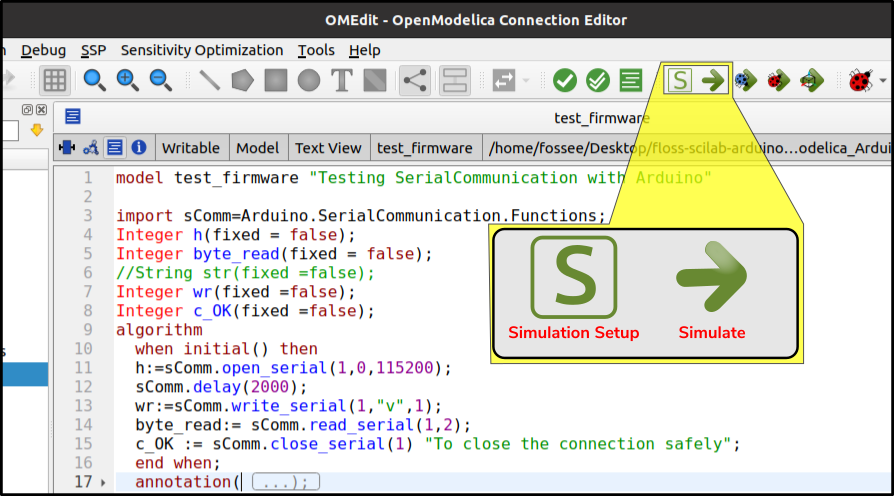
\includegraphics[width=\textwidth]{\LocSWfig/om-simulate.png}
      \caption{Simulating a model in OMEdit}
      \label{om-simulate}
\end{figure}

\begin{figure}
      \centering
      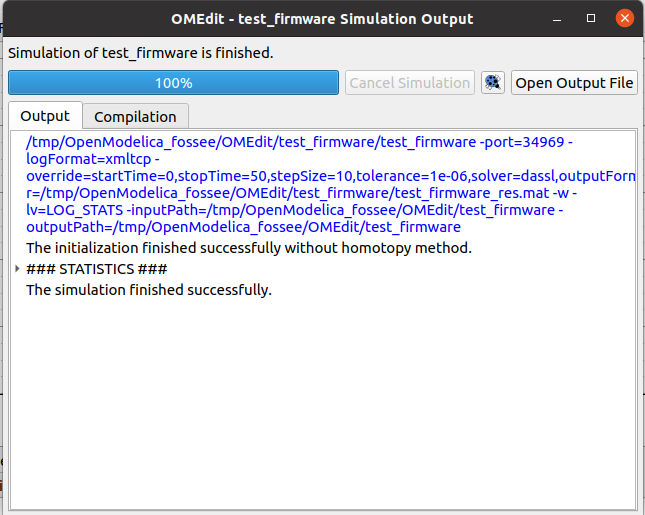
\includegraphics[width=\textwidth]{\LocSWfig/om-sim-success.png}
      \caption{Output window of OMEdit}
      \label{om-sim-success}
\end{figure}

As shown in \figref{om-sim-success}, OMEdit displays the message that "The 
Simulation finished successfully". Had there been any error in simulating the model, 
we would not have received this message. 


\subsection{OpenModelica Arduino toolbox}\label{sec:load-om-toolbox}
OpenModelica, by default, does not have the capability to connect to Arduino. 
All such add-on functionalities are added to OpenModelica using toolboxes.  
The OpenModelica Arduino toolbox can be found inside {\tt Origin/tools/\\openmodelica/windows} or {\tt Origin/tools/openmodelica/linux} directory,
see \fnrefp{fn:file-loc}.  Use the one depending upon
which operating system you are using. The OpenModelica codes for various
experiments mentioned throughout this book can be found in {\tt Origin/user-code} directory. The {\tt user-code} directory will have
many sub-directories as per the experiments. 

Let us now see how to load the OpenModelica Arduino toolbox. 
\begin{enumerate}
      \item First launch OMEdit. On a Windows system, one may start/launch
            OMEdit from the Start menu. On a Linux system, one has to
            start OMEdit through a terminal, as
            explained in section \ref{openmodelica-install-linux}.
      \item After launching, we have to load OpenModelica-Arduino
            toolbox. To do so, go to the menu bar of OMEdit. 
            Click on {\tt File} and then click on
            the {\tt Open Model/Library File(s)} option as shown in \figref{om-model-open}.
      \item Navigate to {\tt Origin/tools/openmodelica/windows} or {\tt Origin/tools/\\openmodelica/linux}, as the case maybe.
            Select {\tt Arduino.mo} and \\{\tt test\_firmware.mo}, and click Open. The toolbox should now be loaded and available for use. 
      \item \label{itm:library} We will check whether the toolbox has been loaded successfully or not. 
            In OMEdit, under Libraries Browser, look for three new libraries: Arduino,
            Modelica\_Synchronous, Modelica\_DeviceDrivers, and one model test\_firmware.mo. 
            If you are able to view these files, it means that OpenModelica-Arduino toolbox has been loaded successfully. 
            Please note that each time you launch OMEdit, you need to load this toolbox for
            performing the experiments. 
      % \item The {\tt test\_firmware.mo} in the step \ref{itm:library} is the same file which has been mentioned in \secref{om-firmware}.
            % While following \secref{om-firmware}, the readers are advised to execute (or simulate) this file (or model). 
      \item \label{itm:locate} Now, we will locate the models for running the experiments in the upcoming chapters. 
            Under Libraries Browser, click on the arrow before Arduino to see the 
            contents inside this package. Next go to SerialCommunication -> Examples. 
            Under Examples, you will find the list of experiments like led, push, etc., 
            as shown in \figref{om-examples-toolbox}.
      \item \label{itm:simulate} For running the experiments of a particular chapter, click on the corresponding 
            experiment's name. Subsequently, you will find a list of experiments which you can 
            simulate one by one, as explained in \secref{OpenModelica-code-execution}.
      \item For each of the experiments using OpenModelica given in the upcoming chapters, the readers 
            are advised to locate the corresponding model by following the steps
            numbered \ref{itm:locate} and \ref{itm:simulate} and simulate it.  
\end{enumerate}



\begin{figure}
      \centering
      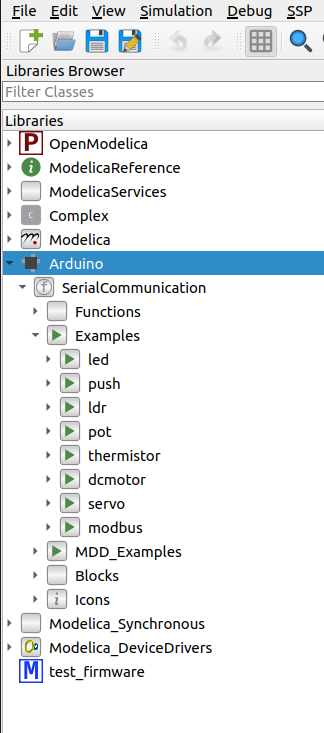
\includegraphics[width=\smfig]{\LocSWfig/om-toolbox-loaded.png}
      \caption{Examples provied in OpenModelica-Arduino Toolbox}
      \label{om-examples-toolbox}
\end{figure}

%%%%%begin OpenModelica code

\subsection{Firmware}\label{om-firmware}
\lstset{style=mystyle}
\label{sec:test-firmware-OpenModelica}
\addtocontents{cod}{\protect\addvspace{\codclr}}
We have provided an OpenModelica code/model to check whether the firmware has been
properly installed.  That code/model is listed below. Please ensure that 
you have uploaded the Arduino firmware given 
in \ardref{ard:firmware} on the \arduino\ board.


\begin{OpenModelicacode}
      \mcaption{An OpenModelica code to check whether the firmware is properly installed
            or not}{An OpenModelica code/model to check whether the firmware is properly installed
            or not.  Available at \LocFIMOpenModelicabrief{test\_firmware.mo}. Locate this file 
            inside OpenModelica-Arduino toolbox, as explained in \secref{sec:load-om-toolbox}. Simulate this code/model by following the steps 
            given in  \secref{OpenModelica-code-execution}. If the simulation is
            successful, you should expect an output window in OMEdit as shown in 
            \figref{om-sim-success}.}
      \label{OpenModelica:test-firmware}
      \lstinputlisting{\LocFIMOpenModelicacode/test_firmware.mo}
\end{OpenModelicacode}

%%%%%end OpenModelicamo
